%versi 2 (8-10-2016)
\chapter{Landasan Teori}
\label{chap:teori}

Pada Bab ini akan dijelaskan dasar-dasar teori tentang Big Data, Data Stream beserta contoh-contohnya, \textit{Apache Spark,} \textit{Spark Streaming}, \textit{Flume}, \textit{Kafka}, dan \textit{Twitter Analytics}. Serta Bahasa pemorgraman yang akan digunakan yaitu\textit{ Scala}.

\section{Big Data}
\textit{Big Data} merupakan data yang melebihi kapasitas pemrosesan dari sistem basis data konvensional. Data Tersebut berukuran terlalu besar, tumbuh dengan sangat cepat, memiliki banyak variasi tipe data, dan tidak cukup pada arsitektur basis data konvensional.

\textit{Big Data} memberikan dua kegunaan untuk sebuah organisasi, yaitu untuk keperluan analisis dan keperluan bisnis. \textit{Big Data} dapat dianalisis untuk mendapatkan informasi seperti hubungan antar pelanggan. Hal ini dapat dilihat dari hasil analisis transaksi setiap pelanggan, graf sosial, dan graf geografis.

suatu set data dapat dikatakan sebagai big data jika set data tersebut memenuhi salah satu dari lima karakteristik big data. Kelima karakteristik \textit{Big Data} yang sering disebut dengan 5V adalah \textit{volume,velocity, variety, veracity, dan value}.

\begin{enumerate}
	\item{\textit{Volume} \newline
	\textit{volume} merupakan istilah untuk menggambarkan ukuran dari data. Data dengan ukuran 		besar mempunyai kebutuhan penyimpanan dan pemrosesan yang berbeda serta tambahan dalam 			persiapan, pengolahan pemrosesan data. Data berukuran besar tersebut dapat berasal dan 			transaksi online, eksperimen penelitian ilmiah, sensor, dan media sosial.
	}
	
	\item{\textit{Velocity} \newline
	\textit{Velocity} dari data merupakan waktu yang diperlukan untuk melakukan pengolahaan 		data ketika data tersebut masuk ke penyimpanan. Untuk menangani data yang masuk dengan 			cepat, perusahaan atau organisasi memerlukan solusi pemrosesan data yang elastis dan 			terbuka, dan sesuai.
	
	Kecepatan dari data tidak selalu tinggi dan tergantung pada sumber data. Kecepatan data 		dapat dipertimbangkan ketika data berukuran besar dan dapat dihasilkan dalam waktu yang 		singkat. Seperti; 350.000 cuitan, 300 jam video, 171 juta surat elektronik, dan 330 			\textit{gigabytes} sensor.
	
	}
	
	\item{\textit{Variety} \newline
	\textit{Variety} atau variasi data mengacu pada banyaknya format dan tipe data yang perlu 		didukung oleh solusi \textit{Big Data}. Variasi data ini merupakan tantangan bagi yang 			ingin melakukan integrasi, transformasi, pemrosesan, dan penyimpanan data.
	}
	
	\item{\textit{Veracity} \newline
	\textit{Veracity} mengacu pada kualitas atau akurasi data. Data yang masuk akan diperiksa 		untuk menentukan kualitas dan menghindari adanya data yang tidak valid serta menghilangkan 		\textit{Noise}. Data yang masuk tersebut dapat terdiri dari sinyal dengan informasi 			tersimpan dan \textit{noise} dari suatu set data. Noise tersebut tidak menyimpan informasi 		bermakna dan tidak bernilai. Oleh karena itu, data dengan perbandingan sinyal terhadap 			noise yang besar, memiliki veracity yang lebih besar. 	
	}
	
	\item{\textit{Value} \newline
	\textit{Value} atau nilai didefinisikan sebagai kegunaan data tersebut bagi perusahaan atau 	organisasi. Karakteristik value berhubungan \textit{linear} dengan karakteristik 				\textit{veracity} karena besarnya veracity tersebut menentukan besarnya nilai yang dimiliki 	suatu data dapat bernilai hanya pada rentang waktu tertentu saja dan tidak bernilai di luar 	rentang waktu tersebut.
	}
\end{enumerate}

\textit{Big Data} yang diolah dapat dihasilkan oleh manusia maupun mesin. Data yang dihasilkan manusia berapa hasil interaksi antara manusia dengan sistem. Data yang dihasilkan oleh mesin dapat berupa hasil dari perangkat lunak maupun perangkat keras sebagai respon dari aktivitas dunia nyata. Data yang dihasilkan tersebut dapat dikelompokan menjadi tiga tipe dasar yaitu; data terstruktur, data tidak tersturktur, dan data semi terstruktur.

\begin{enumerate}
	\item{Data Terstruktur \newline
	Data Terstruktur adalah data yang dimodelkan dalam sebuah model data atau skema data dan 		biasanya disimpan dalam bentuk tabel relasional. Data Tersebut digunakan untuk melihat 			hubungan antar entitas sehingga pada umumnya tersimpan dalam basis data relasional. Data 		terstruktur biasanya dihasilkan dari aplikasi perusahaan dan sistem informasi. Data 			terstruktur tidak memerlukan pertimbangan khusus. Terkait penyimpanan maupun pemrosesan 		karena basis data sudah mendukung tipe data terstruktur.
	}
	
	\item{Data Tidak Terstruktur \newline
	Data Tidak terstruktur merupakan data yang tidak dimodelkan dalam model data atau skema 		data. Sebagian besar dari data perusahaan merupakan data yang tidak terstruktur. Data tidak 	terstruktur pada umumnya berupa file teks atau media yang masing-masing tidak tergantung 		pada file-file lain. Oleh karena itu, pengolahaan data tidak terstruktur memerlukan 			penanganan khusus. contoh: video memerlukan \textit{coder} dan \textit{encoder}
	}
	
	\item{Data Semi Terstruktur \newline
	Data semi terstruktur mempunyai struktur tertentu dan konsisten, tetapi tidak bersifat 			relasional. Struktur data pada tipe ini berupa struktur hirarkis atau dalam bentuk graf. 		umumnya berbentu XML atau JSON. Adanya struktur dalam data membuat data semi terstruktur 		lebih mudah untuk diproses dibandingkan data tidak terstruktur.
	}
	
\end{enumerate}
\label{sec:Big Data} 
 


\section{Big Data Stream}
\textit{Data Stream} adalah urutan rekaman atau kejadian (\textit{events}) yang tidak pernah
 berhenti. Serangkaian \textit{data stream} bersifat tidak terbatas dan akan terus dihasilkan
 \textit{(in-motion)} sedangkan waktu dan tempat yang dialokasikan untuk mengolah data terbatas.
 Selain itu, sifat khusus dari \textit{data stream} adalah interaksi yang terbatas dengan sumber
 data, \textit{data stream} hanya bisa menerima data dari sumber dan tidak bisa mengirim informasi
  kembali dan data yang dihasilkan hanya bisa di akses dan diproses sekali saja sebelum ditumpuk dan
 dikumpulkan di tempat penyimpanan. Sehingga, hanya satu atau beberapa elemen terbaru saja yang bisa
 diproses.
 
 \textit{Big Data Stream } adalah gabungan dua sifat dari \textit{Big Data} dan \textit{Data Stream}
 . Selain memiliki atribut-atribut \textit{Big Data} yang besar, berkembang dengan sangat cepat,
 dan bervriatif. \textit{Big Data Stream} terus menerus dihasilkan sedangkan watku dan tempat untuk
 mengolah data tersebut sangat terbatas. 
		
\textit{Data stream} banyak digunakan untuk proses agregasi, korelasi, dan 					
\textit{filtering} secara \textit{real-time}. \textit{Data Stream} memungkinkan pengguna 				
untuk melihat \textit{insights}, menganalisisnya, dan menarik kesimpulan dari 							
\textit{insights} tersebut. Beberapa contoh analisis adalah; memantau informasi dari suatu 				
sosial media seperti \textit{twitter} untuk mendapatkan informasi untuk mengetahui tingkah 				
pengguna, memantau aktivitas web dengan mencatat pembaharuan \textit{web logs} setiap 					
detiknya, mendeteksi anomali dari suatu jaringan atau sensor yang terus menerus mengirimkan 			
data untuk dianalisis. Contoh beberapa kasus nyata adalah:

\begin{itemize}
	\item institusi keuangan yang memantau perubahan pasar saham. Sehingga bisa mengubah 			
	portofolio berdasarkan batasan batasan tertentu(menjual saham ketika saham mencapai titik 		
	nilai tertentu)
	\item Memantau suatu jaringan listrik berdasarkan \textit{througput} dan akan memberi 			
	peringatan jika melebihi batas tertentu.
	\item Kantor berita yang menggunakan \textit{clickstream} dari berbagai platform untuk 			
	memperkaya data dengan informasi demografik sehingga bisa merekomendasikan artikel ke 			
	pembaca yang relevan.
	\item perusahaan \textit{e-commerce} menggunakan data stream untuk melihat apakah ada 			
	anomali pada datastream dan akan mengirimkan peringatan jika terjadi anomali.
\end{itemize}



\subsection{Pengertian Stream Processing}
Stream Processing adalah proses yang dirancang untuk mengatasi untaian data yang tidak
terbatas atau tidak memiliki awalan dan akhiran yang jelas. Stream Processing menawarkan pem-
rosesan data dengan latency yang rendah dan hasil yang spekulatif. Untuk memproses suatu data,
stream processing mempunyai dua dimensi penting yaitu; cardinality dan constitution. cardinality
adalah ukuran dari data tersebut; terbatas (bounded) atau tidak terbatas (unbounded). Constitution
adalah bagaimana data ditampilkan; adalah bagaimana data ditampilkan; tabel yang menampilkan
data secara menyeluruh seperti SQL atau potongan-potongan le pada HDFS seperti Map Reduce.

Walaupun Stream Processing menawarkan Latency yang rendah, namun hasil dari data yang diproses
kurang akurat. Hal ini disebabkan karena Stream Processing menggunakan algoritma pendekatan.
Salah satu cara mengatasi masalah ini adalah dengan perancangan arsitektur Lambda. Pembahasan 
arsitektur Lambda dan Kappa akan dibahas lebih lengkap di 2.2.4. Stream processing memodelkan waktu 
menjadi dua domain; Event time dan Processing Time. \textit{Event-Time} adalah waktu saat data 
sedang dihasilkan. Setiap data yang dihasilkan akan diber \textit{time stamp} agar semua data dari 
sumber yang sama bisa diurutkan secara kronologis. \textit{Event-time} digunakan
diantaranya untuk menggolongkan perilaku pengguna dari waktu ke waktu.Processing time adalah
waktu ketika data diobservasi pada Stream-Processing. Secara ideal, \textit{event time} dan 
\textit{processing time} bernilai sama. Artinya, sistem langsung mengobservasi data saat data itu 
sedang dihasilkan. Namun pada nyatanya, nilai processing time dan event time tidak selalu sama 
karena dipengaruhi sumber data, waktu ekseskusi, dan performa mesin hardware. Hubungan antara event 
time dan processing-time bisa dilihat di Gambar 1:

 

\subsection{Pemodelan Stream Processing} 

Pada \textit{Stream Processing} waktu dimodelkan menjadi dua domain yaitu; \textit{Event Time} dan 
\textit{Processing Time}.\textit{Event Time} digunakan diantaranya untuk menggolongkan perilaku pengguna dari waktu ke waktu,  aplikasi tagihan, mendeteksi suatu anomali yang terjadi. Secara ideal, \textit{event time} dan  \textit{Processing time} bernilai sama. Artinya, sistem langsung mengobservasi data saat data itu sedang dihasilkan.
 
Tetapi pada nyatanya tidak semulus itu, nilai \textit{event time} dan 
\textit{processing time} tidak selalu sama karena dipengaruhi sumber data, waktu eksekusi, dan 
performa mesin serta \textit{hardware}. Hubungan antara \textit{event time} dan \textit{processing 
time} bisa dilihat pada gambar

\begin{figure}[H] 
	\centering  
	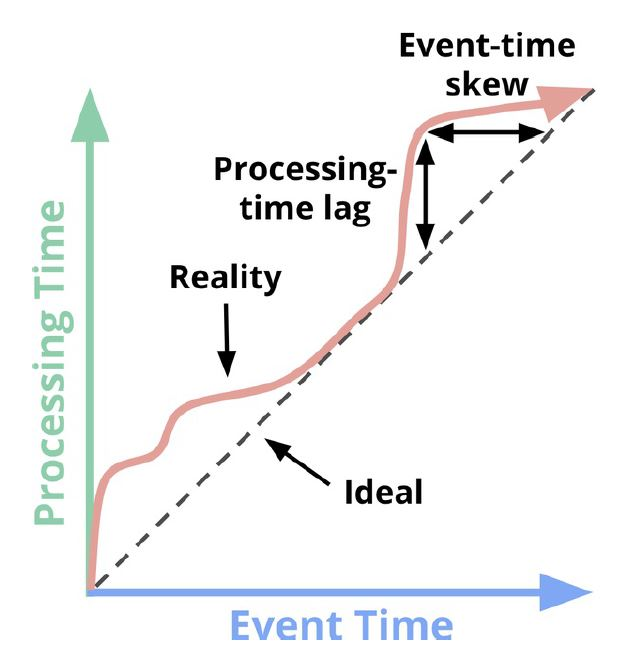
\includegraphics[scale=0.5]{1-processing-event-relationship}  
	\caption[Gambar Pemetaan {\it Time-Domain}]{Pemetaan {\it Time-Domain}} 
	\label{fig:processing-events relationship} 
\end{figure} 
 
Sumbu X adalah \textit{event time} atau completeness dalam sistem. Sumbu Y adalah Processing time 
waktu jam biasa yang diamatai oleh sistem data processing ketika sedang dieksekusi. Processing-time 
lag adalah jarak vertikal antara garis ideal dengan garis merah yang menunjukan ada berapa banyak
waktu delay yang sedang diobservasi di antara kejadian pada waktu tertentu dan kapan delay itu
terjadi. event-time skew adalah garis horizontal dari garis ideal dengan garis merah yang menunjukan
banyaknya distribusi data di pipeline pada saat itu dan menunjukan seberapa ketinggalan suatu pipeline dari pipeline ideal. 

\subsection{Pola Pemrosesan Data Stream}
Pola-pola teknik pemrosesan stream procesing dibagi menjadi dua yaitu batch dan streaming.
Pola yang tergolong ke dalam batch tidak dirancang untuk data yang tidak terbatas. Tetapi pemrosesan
data tidak terbatas bisa dilakukan dengan membagi dataset menjadi beberapa bagian yang berisi
potongan-potongan dari dataset tersebut yang lebih kecil dan terbatas. Sehingga bisa diproses dengan
batch processing. Beberapa jenis batch processing adalah \textit{fixed windows} dan 
\textit{Session}:



	\subsubsection{Fixed Windows}
	\textit{Fixed Windows} adalah pola pemrosesan yang paling umum. \textit{Fixed Windows} 			
	memproses dataset tidak terbatas menggunakan mesin \textit{batch} yang dijalankan 				
	dengan cara membagi input data ke beberapa \textit{window} dan memproses setiap  				
	\textit{window} tersebut secara terpisah. proses ini dilakukan secara berulang-ulang. 			
	Seperti pada gambar 2.2. Metode ini digunakan untuk data yang berbentuk logs karena 			
	data bisa ditulis pada directory dan hirarki file dengan nama yang sama dengan window.			
	Jika data terkena delay gara-gara partisi \textit{network} perlu dilakukan mitigasi 			
	yang memperlambat proses sampai semua data terkumpul ketika data datang terlambat 				
	sistem telah memproses seluruh \textit{batch} sebelum dipindahkan ke \textit{windows}.
		
		\begin{figure}[H] 
		\centering  
		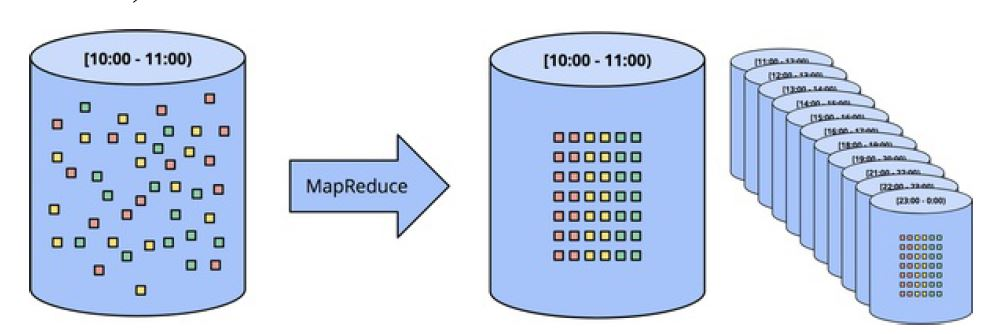
\includegraphics[scale=0.5]{3-fixed-windows}  
		\caption[Gambar {\it fixed-windowa}]{\textit{data processing} dengan 					
		menggunakan fixed window} 
		\label{fig:processing-events relationship} 
		\end{figure} 
	
	
	\subsubsection{Session} 
	memiliki cara kerja yang hampir sama dengan \textit{fixed windows} bedanya pemotongan data 
	dipisah berdasarkan session sehingga pembagian data jadi tidak seimbang data yang sama
	mungkin berakhir di batch berbeda.
	
	Session adalah aktivitas atau periode spesifik yang akan dihentikan bila diselingi oleh 		
	suatu ketidakaktifan  Session dihitung oleh batch processing dan dibagi ke pada seluruh 		
	batch seperti pada gambar 4. Banyaknya split berbanding terbalik dengan latency. Jadi, 			
	bila jumlah split dikurangi maka latency akan menigkat. Sebaliknya jika split 					
	bertambah, latency akan berkurang.
		
		\begin{figure}[H] 
		\centering  
		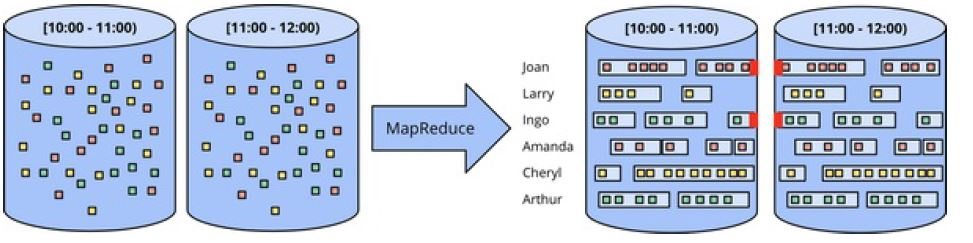
\includegraphics[scale=0.5]{4-session-batch}  
		\caption[Gambar {\it Session-batch}]{{\it Unbounded Data Processing} dengan 					
		\textit{Sessions}} 
		\label{fig:processing-events relationship} 
		\end{figure} 
	

Pola-pola yang dikelompokan menjadi \textit{Streaming}khusus dibangun untuk memproses data tidak terbatas (unbounded). Karena pada kasus nyata banyak data yang tidak teratur atau berbentuk dan tidak sekuensial. Sehingga jika data ingin dianalisis dalam konteks data itu masih baru, harus ada sebuah metode pada pipeline untuk mengurutkan data berdasarkan waktu. Ada empat pola yang digunakan sebagai pendekatan terhadap dataset yang mempunyai karakteristik-karakteristik ini yaitu; \textit{filtering}, \textit{approximation algorithm}, dan \textit{windowing}.


	\subsubsection{filtering}
	\textit{filtering} adalah operasi mendasar dan dilakukan secara \textit{Time-Agnostic} yang 
	memilah data yang masuk. Pola \textit{Time-Agonstic} digunakan untuk kasus-kasus dimana waktu 
	tidak relevan. Artinya, semua logika dan informasi pada data yang relevan ada pada data dan 
	yang lebih menentukan relevansi dari suatu data adalah urutan kedatangan data 
	tersebut. Jadi, pola ini hanya membutuhkan streaming engine yang mendukung pengiriman 
	data yang sederhana karena itu semua sistem streaming bisa menggunakan pola Time-
	AgnosticSistem melihat setiap rekord yang datang dan melihat apakah domain data 	
	sama dengan domain tujuan. Bila tidak data akan dibuang karena itu proses ini hanya 			
	bergantung pada urutan kedatangan data bukan dari \textit{event-time}.
	
	\begin{figure}[H] 
	\centering  
	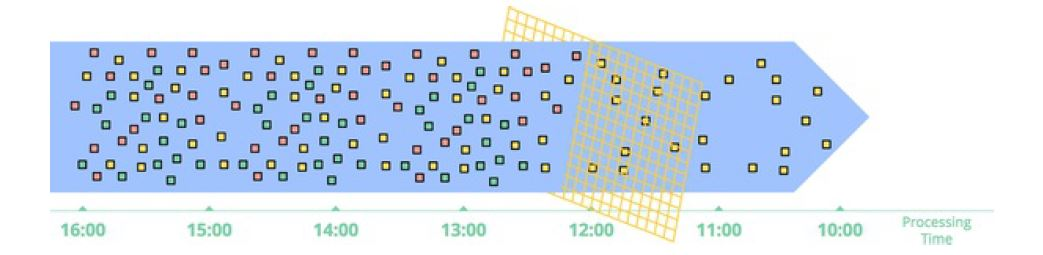
\includegraphics[scale=0.5]{8-Filtering-Unbounded-data}  
	\caption[Gambar {\it Filtering-unbounded-data}]{\textit{Filtering data}} 
	\label{fig:processing-events relationship} 
	\end{figure} 
	
	proses di atas adalah proses \textit{filtering data} dari kumpulan data yang
	heterogen menjadi homogen dengan tipe yang sama dan diletakan pada klaster yang sama.salah
	satu cara untuk mengelompokan data yang bersifat sama adalah dengan melakukan \textit{Inner 
	Join}.\textit{Inner Join} adalah salah satu bagian dari filtering dimana proses menggabungkan 
	dua sumber data yang tidak terbatas. Jika ada suatu data datang sistem akan menyimpan data 
	tersebut ke \textit{persistent state} ketika data berikutnya datang sistem akan 
	menggabungkan data tersebut dengan data yang ada di persistent state.
	
	\begin{figure}[H] 
	\centering  
	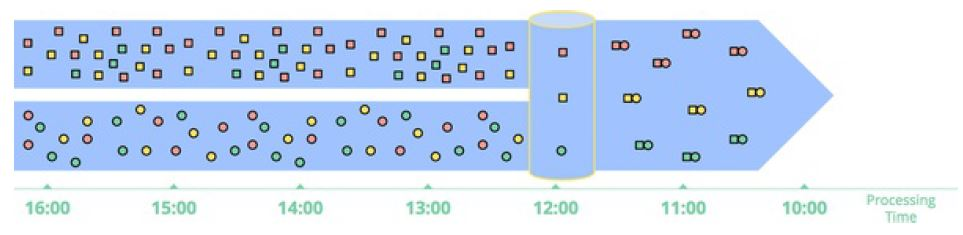
\includegraphics[scale=0.5]{6-inner-join}  
	\caption[Gambar {\it inner-join}]{\textit{inner join} pada \textit{unbounded data}} 
		\label{fig:processing-events relationship} 
		\end{figure} 
	
	
	\subsubsection{Approximation Algorithm}
	\textit{Approximation algorithm} adalah algoritma pendekatan yang menerima input data tidak 
	terbatas dan mengelompokan data tersebut menjadi berdekatan jika memiliki sesuatu kesamaan. 
	sperti pada gambar 2.5. 
	Algoritma pendekatan ini memang dirancang untuk data tidak terbatas. Tetapi, 
	algortima pendekatan merupakan algoritma yang rumit sehingga algoritma pendekatan susah 
	untuk dipanggil ketika dibutuhkan, dan pendekatan dari algoritma ini cenderung terbatas. 
	
	\begin{figure}[H] 
	\centering  
	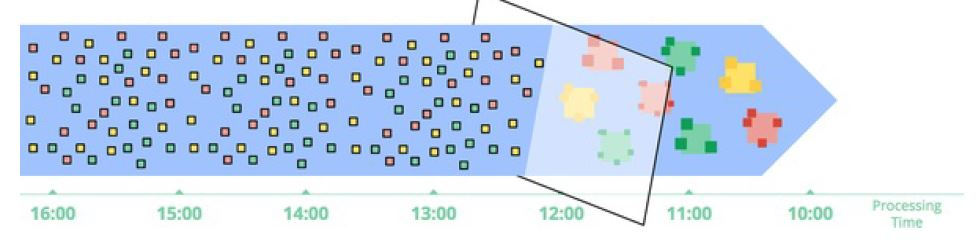
\includegraphics[scale=0.5]{5-approximation-algorithm}  
	\caption[Gambar {\it approximation-algorithm}]{Algoritma pendekatan pada \textit{unbounded 		
	data}} 
	\label{fig:processing-events relationship} 
	\end{figure} 
	
	Data dijalankan melewati algoritma yang kompleks dan menghasilkan data output yang 		
	terlihat lebih mirip hasil yang diinginkan. Algoritma pendekatan langsung memproses data yang 
	datang karena itu melibatkan \textit{processing time}. \textit{Processing-time} digunakan 
	algoritma sebagai pengecek  \textit{error} pada data dengan membaca waktu urutan kedatangan 
	dari data.
	
	
	\subsubsection{Windowing}
	\textit{Windowing} adalah fungsi menerima \textit{data source} sebagai input. Lalu, membagi 	
	data tersebut menjadi beberapa bagian dan memberi batasan pada potongan data tersebut. Bisa 		
	dilihat pada gambar 2.6. Windowing memiliki dua variasi \textit{Fixed Windows} dan 				
	\textit{Sliding Windows} 		
	
	\begin{figure}[H] 
	\centering  
	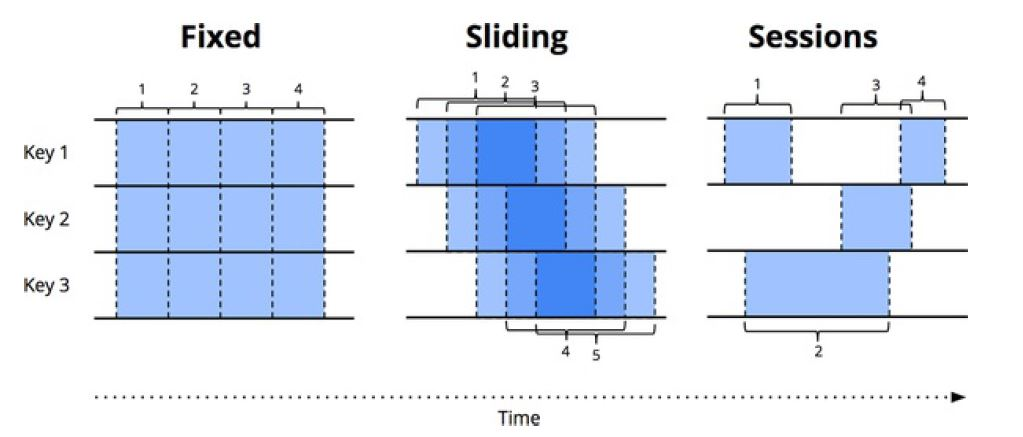
\includegraphics[scale=0.5]{7-Windowing}  
	\caption[Gambar {\it Windowing}]{Teknik Windowing} 
	\label{fig:processing-events relationship} 
	\end{figure}
	 
	Windowing memiliki beberapa pola yang sering digunakan beberapa contohnya adalah:
	\begin{itemize}
		\item{Fixed Windows (Tumbling Windows)bekerja Seperti Fixed windows pada batch processing. 
		Fixed windows membagi waktu menjadi segmen-segmen dengan ukuran yang tetap. Seperti pada 
		gambar 2.6. Segmen untuk fixed window diterapkan secara seragam pada seluruh dataset. 
		Pembagian segmen dengan ukuran yang sama disebut aligned window. Tetapi, terkadang window 
		tidak dibagi dengan ukuran yang sama. Dalam beberapa kasus, pembagian data bergantung pada 
		ukuran dataset dan bervariasi tiap dataset. Pembagian waktu yang tidak merata, unaligned 
		window, membantu meratakan penyebaran waktu penyelesaian.
		}
		
		\item{Sliding Windows(Hoping Windows)adalah fixed window yang lebih umum. Sliding windows 
		memiliki panjang dan periode yang tetap. Jika periode lebih kecil dari length maka terjadi 
		overlap pada windows. Jika periode sama dengan waktu maka window akan menjadi fixed window. 
		Jika periode lebih besar dari length maka akan menjadi sampling window yang hanya 
		akan melihat suatu subset data dengan waktu yang lama. Seperti pada gambar 2.6
		
		}
		
		\item{Dynamic sessions biasanya digunakan untuk menganalisa perilaku pengguna secara 
		berkala dengan megelompokan suatu rantaian peristiwa yang berhubungan. contohnya adalah 
		berapa banyak video yang ditonton oleh pengguna dalam sekali duduk. Panjang dari suatu sesi 			tidak bisa ditentukan terlebih dahulu. Panjang sesi tergantung dari seberapa banyak 			
		data yang terlibat. Dynamic Session merupakan salah satu penerapan unaligned window 			
		karena untuk setiap session subset pada suatu dataset tidak pernah identik.
		
		} 
	\end{itemize}
	
	Selain itu Windowing bekerja dengan dua cara berbeda. Seperti \textit{Processing-time 
	Windowing} dimana Sistem menyimpan sementara data yang datang pada window untuk beberapa saat 
	sampai processing time telah lewat. Contohnya; misalkan ada fixed windows dengan durasi 5 			
	menit, sistem akan menyimpan sementara data selama lima menit waktu pemrosesan. Lalu, 			 
	sistem akan mengirim data yang telah diobservasi selama lima menit tersebut ke 				 
	\textit{downstream} untuk diproses.\\
	 	
	Proses windowing ini sangat simpel dan implementasinya mudah karena sistem tidak harus 		 
	mengatur data sesuai waktu. data hanya akan disimpan sementara ketika datang dan 				 
	langsung dilempar ke downstream ketika processing time selesai. Karena sistem bisa 			 
	mengetahui semua input karena telah dilihat oleh window. Sehingga sistem bisa dengan 			 
	baik memprediksi kapan suatu window akan selesai. metode yang kedua adalah \textit{Event-time 
	Windowing} Event-time Windowing digunakan ketika sistem mengobservasi sumber data yang tidak 
	terbatas dalam potongan-potongan data yang terbatas berdasarkan kapan data itu terjadi.
	 	
 

\subsection{Arsitektur Stream Processing}

\subsubsection{Lambda Architecture}
Arsitektur Lambda adalah teknik pemrosesan data yang bisa menangani data yang besar dengan cara mneggabungkan metode batch dan stream processing. Teknik ini menyeimbangkan antara latency, throuhput, dan fault-tolerance dengan menggunakan batch processing yang menyediakan penyimpanan data yang akurat dan komperhensif. Juga memanfaatkan stream processing agar mendapat data tidak terbatas secara realtime.

Banyak perusahaan yang menggunakan metode stream procesing untuk memprediksi updates dari model dan menyimpan event yang berbeda yang digunakan sebagai bahan untuk memprediksi. Untuk menangani kejadian seperti itu, Arsitektur Lambda memilki tiga layer; \textit{Batch layer}, \textit{speed layer (stream layer)}, dan \textit{Serving layer}.
	\begin{figure}[H] 
	\centering  
	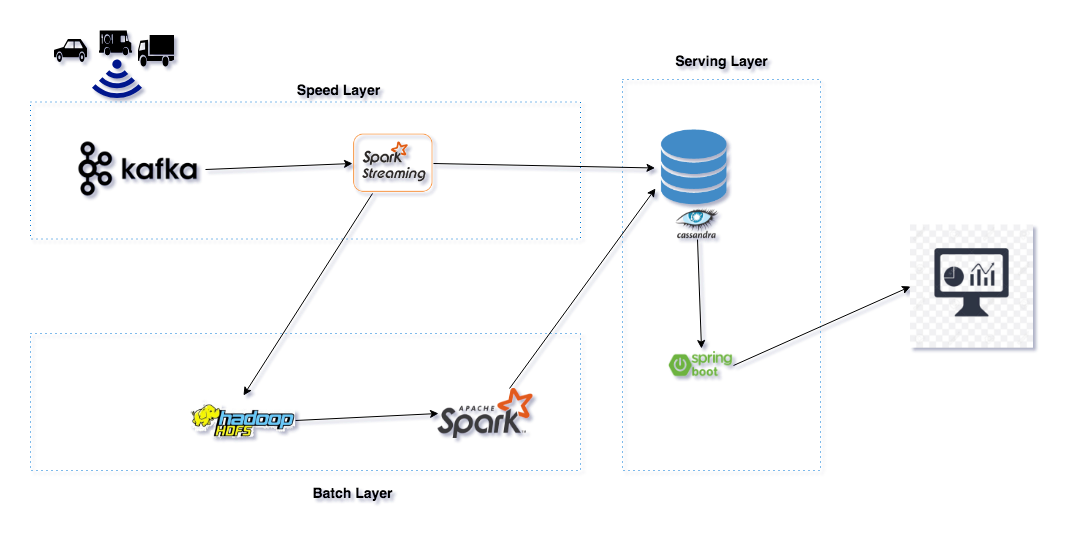
\includegraphics[scale=0.45]{lambda-architecture}  
	\caption[Gambar Arsitektur { \it Lambda}]{Arsitektur {\it Lambda}} 
	\label{fig:processing-events relationship} 
	\end{figure}
	
\begin{itemize}
	\item[]{\textit{batch layer}\newline
	layer ini terlebih dahulu memproses data dengan menggunakan sistem terdistribusi yang bisa 		
	menangani data yang besar. tujuan dari batch layer adalah untuk meningkatkan akurasi dengan 	
	cara memproses semua data yang ada ketika membangun view. Artinya, batch layer bisa 			
	memperbaiki error pada data dengan memproses data kembali berdasarkan dataset yang sudah 		
	lengkap.

	Setiap data yang terus menerus datang ke sistem akan diteruskan ke batch layer dan stream 		
	layer secara bersamaan. Data Stream yang baru masuk ke batch layer langsung diproses pada 		
	data lake. Data disimpan pada data lake menggunakan in-memory database atau long term 			
	persistent database seperti NoSQL. Data akan diproses menggunakan MapReduce atau machine-		
	learning. Apache hadoop digunakan di layer ini karena memiliki throughput yang paling 			
	tinggi.	
	}
	
	\item[]{\textit{Speed Layer(Stream Layer)}\newline
	Layer ini memproses data stream secara real-time tanpa memperdulikan completeness atau 			
	akurasi dari data. layer ini mengurangi throughput untuk mengurangi latency. Sehingga data 		
	yang terbaru bisa langsung dilihat. Speed layer digunakan untuk mengisi jarak yang 				
	disebabkan oleh batch layer dengan memberikan informasi tentang data terkini. View yang 		
	dihasilkan dari layer ini belum tentu akurat namun bisa langsung dilihat dan diakses. Data 		
	yang lebih akurat akan disediakan dan diganti nanti oleh hasil data yang telah diolah oleh 		
	batch layer ketika sudah tersedia.
	}
	
	\item[]{\textit{Serving Layer}\newline
	Output dari batch dan Speed layer diteruskan dan disimpan di layer ini dan proses ad-hoc 		
	queries akan dilakukan di layer ini dengan mengembalikan views dari data yang telah 			
	diproses.

	Arsitektur Lambda dapat dianggap sebagai arsitektur pemrosesan data yang real-time. Seperti 	
	disebutkan di atas, dapat menahan kesalahan serta memungkinkan skalabilitas. Arsitektur ini 	
	menggunakan fungsi-fungsi batch dan stream lalu menambahkan data baru ke penyimpanan utama 		
	sambil memastikan bahwa data yang ada akan tetap utuh. Perusahaan seperti Twitter, Netflix, 	
	dan Yahoo menggunakan arsitektur ini untuk memenuhi kualitas standar layanan.

	}
\end{itemize}

Keuntungan dari Arsitektur Lambda antara lain adalah; \textit{Batch Layer} dari arsitektur ini mengatur histori data dengan penyimpanan terdistribusi yang \textit{fault tolerant} yang mana akan memperkecil terjadinya error walaupun sistem \textit{crash}, seimbang antara kecepatan dan keandalan, Scalable dan fault tolerant untuk data processing. Tetapi, arsitektur ini memiliki kelemahan yaitu; penerapan yang cukup sulit karena melibatkan \textit{batch} dan \textit{stream processing}, memproses setiap batch pada beberapa \textit{cycle} tidak menguntungkan untuk beberapa skenario, data yang dimodelkan dengan arsitektur ini susah untuk dimigrasi dan diorganisir ulang.

\subsubsection{Kappa Architecture}
\textit{Kappa Architecture} adalah simplifikasi dari arsitektur lambda. Susunan arsitektur ini hampir sama dengan sistem arsitektur lambda namumn tidak memiliki \textit{batch layer}. 
Untuk mengganti \textit{batch processing} data langsung diteruskan ke sistem streaming. 
Arsitektur ini digunakan model data berupa; beberapa \textit{event} atau \textit{query} data dicatat 
dalam suatu antrian untuk disesuaikan dengan penyimpanan atau riwayat sistem file terdistribusi, 
urutan \textit{event} dan \textit{query} tidak ditentukan sebelumnya, platform \textit{stream 
processing} dapat berinteraksi dengan basis data kapan saja. model ini sangat \textit{resilient} dan 
bisa menangani beberapa terabyte data untuk penyimpanan yang diperlukan untuk setiap sistem node 
yang mendukung replikasi.


Skenario data yang disebutkan di atas ditangani oleh \textit{Apache kafka} yang cepat, toleran 
terhadap kesalahan dan dapat diskalakan secara horizontal. Hal ini memungkinkan mekanisme yang lebih 
baik untuk mengatur aliran data. kerena kontrol yang seimbang pada \textit{stream processing} dan 
database maka hal ini memungkinkan aplikasi untuk bekerja sesuai ekspektasi.Kafka menyimpan data 
yang diminta untuk jangka waktu yang lebih lama dan meayani \textit{queries} analog dengan 
menautkannya ke posisi yang sesuai dari log yang disimpan. Manfaat dari arsitektur ini adalah bisa 
mempertahankan sejumlah besar data untuk menyelesaikan \textit{queries}

keuntungan dari arsitektur ini adalah dapat digunakan untuk mengembangkan sistem data yang merupakan 
yang tidak membutuhkan \textit{batch layer}, Pemrosesan ulang hanya diperlukan saat kode berubah dan 
dapat digunakan dengan memori tetap,Lebih sedikit sumber daya yang diperlukan karena pembelajaran 
mesin dilakukan secara \textit{real-time}. Tetapi, tidak adanya \textbf{batch layer} dapat 
mengakibatkan kesalahan selama pemrosesan data atau saat memperbarui database yang mengharuskan 
untuk ada pemrosesan ulang atau rekonsilisasi.

\label{sec:Big Data Stream}

\section{Sistem Terdistribusi Hadoop}
\textit{Apache Hadoop} merupakan sebuah \textit{framework} yang bersifat \textit{open-source} untuk menulis dan menjalankan aplikasi terdistribusi untuk mengolah data dalam ukuran besar. Proyek Hadoop disusun dengan tujuan untuk mengatasi masalah skalabitas pada \textit{nutch}, sebuah \textit{open-source crawler} dan mesin pencarian. Hadoop merupakan bagian dari implementasi hasil riset google mengenai sistem file terdistribusi dan komputasi pararel.

Hadoop dapat berjalan di atas klaster mesin-mesin dengan kekuatan pemrosesan yang setara dengan komputer komersial maupun berjalan dengan layanan komputasi \textit{cloud}  yang dapat diakses dengan mudah oleh klien. Sistem terdistribusi Hadoop tidak perlu menggunakan mesin-mesin berspesifikasi tinggi, karena beban pemrosesan akan didistribusikan ke masing-masing mesin di dalam klaster. Sistem tersebut dapat memudahkan pengguna ketika sistem diperlukan untuk pengolahan data dengan ukuran lebih besar, karena penambahaan ukuran data hanya memerlukan tambahan mesin ke dalam klaster dengan spesifikasi yang sama atau mendekati mesin-mesin lain dalam klaster.

Mesin-mesin dalam klaster dapat menjadi lebih ekonomis dibandingkan dengan menggunakan sebuah mesin dengan sepsifikasi yang lebih baik. Hal ini terkait dengan penambahan ukuran data yang akan diproses serta kerusakan perangkat keras yang mungkin terjadi. Hadoop dapat mengatasi kasus kerusakan tersebut tanpa ada kehilangan data, tetapi penggunaan sebuah mesin saja memiliki resiko kehilangan data saat ada kerusakan. selain itu, penggatian sebuah mesin yang rusak di dalam klaster akan memerlukan biaya yang lebih kecil dibanding menggani mesin dengan spesifikasi tinggi.

Hadoop memerlukan pengolahaan data dengan ukuran yang sangat besar, Sehingga pemindahan data berukuran besar tersebut melalui jaringan akan memperlambat jalannya proses. Oleh karena itu, data tersebut diperkecil dengan membagi data tersebut menjadi blok-blok data dan mendistribusikannya ke masing-masing mesin dalam klaster. Kode aplikasi yang merupakan sebuah pekerjaan di lingkungan Hadoop dan berukuran lebih kecil dibandingkan dengan data akan didistribusikan ke dalam mesin-mesin klaster. Dengan demikian, pekerjaan pemrosesan data akan terjadi di setiap mesin di dalam klaster terhadap blok-blok data yang ada pada masing-masing mesin klaster.

\subsubsection{Arsitektur Hadoop}
Sebuah klaster hadoop terdiri dari mesin-mesin yang saling terhubung. Klaster hadoop mempunyai arsitektur master/slave dengan sebuah mesin sebagai master node dan mesin-mesin lain sebagai slave node seperti yang ditunjukan pada gambar. Setiap node tersebut akan mempunyai komponen penyimpanan berupa HDFS dan komponen komputasi berupa MapReduce. Seperti yang ditunjukan pada gambar dapat dilihat bahwa HDFS dan MapReduce pada node mempunyai \textit{daemon} dan tugas yang berbeda dengan komponen HDFS dan MapReduce yang ada pada slave node. Perbedaan tugas-tugas tersebut akan dijelaskan dibagaian.

	\begin{figure}[H] 
	\centering  
	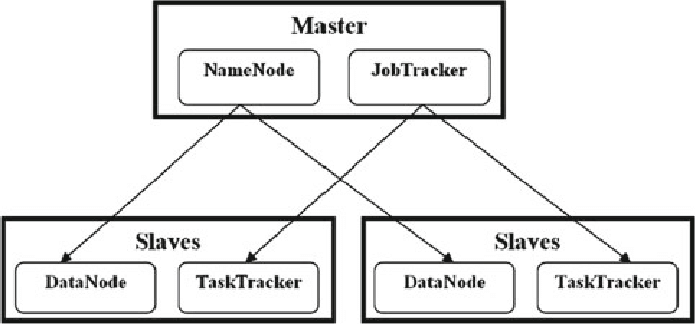
\includegraphics[scale=0.5]{Master-slave}  
	\caption[Gambar Arsitektur { \it Hadoop}]{Arsitektur {\it Hadoop}} 
	\label{fig:processing-events relationship} 
	\end{figure}

\subsubsection{Komponen-Komponen penting Hadoop}
\begin{itemize}
	\item[]{\textbf{\textit{Hadoop Distributed File System}(HDFS)}\newline
		Hadoop distributed file system atau HDFS adalah komponen penyimpanan data dalam Hadoop.
		HDFS dirancang untuk memiliki \textit{throughput} tinggi dan cocok untuk melakukan 						operasi baca dan tulis pada file dengan ukuran yang sangat besar. Untuk mendukung hal 					tersebut, HDFS memanfaatkan ukuran blok data yang besar dan optimasi lokalitas data 					untuk mengurangi input output jaringan. Selain itu, data yang tersimpan di dalam HDFS 					tidak akan hilang ketika ada kerusakan pada salah satu mesin. Hal ini disebabkan adanya 				replikasi untuk setiap blok data yang terdistribusi di dalam klaster. Banyaknya 						replikasi yang terjadi pada awalnya adalah tiga, tetapi angka ini dapat dikonfigurasi 					ulang menjadi lebih sedikit maupun lebih banyak.
		
		\begin{figure}[H] 
		\centering  
		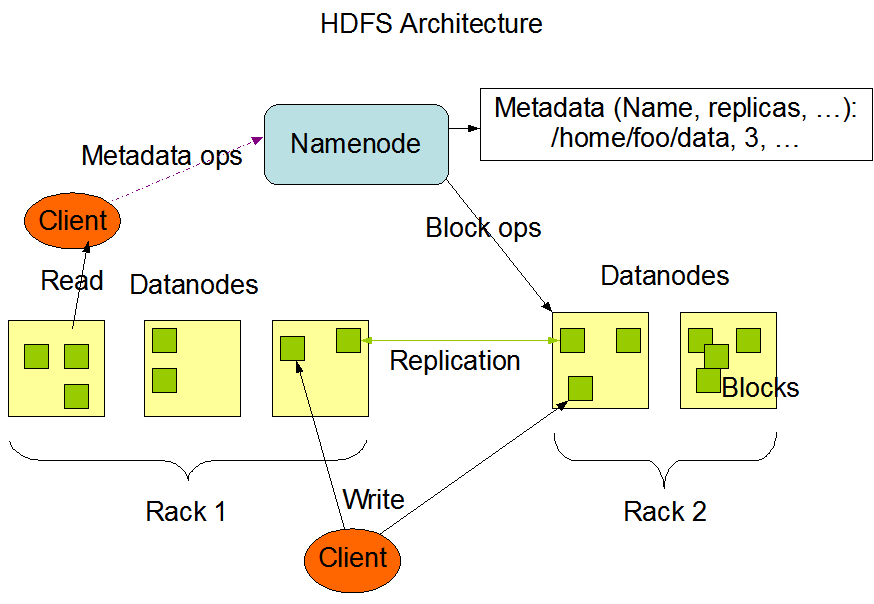
\includegraphics[scale=0.5]{hdfsarchitecture}  
		\caption[Gambar Arsitektur HDFS]{Arsitektur HDFS} 
		\label{fig:HDFS Architecture} 
		\end{figure}
		
		Komponen HDFS pada master node menjalankan sebuah daemon yang disebut dengan NameNode. 					NameNode bertugas untuk mengatur pembagian blok-blok data ke slave node dan mencatat 					lokasi masing-masing blok data tersebut. NameNode Merupakan komponen yang penting dalam 				ekseskusi pemrosesan data dalam klaster. Berbeda dengan Master Node, komponen HDFS pada 				slave node menjalankan daemon yang disebut dengan DataNode. Data Node bertugas untuk 					melakukan proses baca tulis blok-blok data pada file asli yang terdapat sistem file 					lokal. Komunikasi pada awal operasi tulis atau baca terjadi diantara klien dan NameNode 				untuk mendapatkan lokasi blok-blok data yang akan diproses. setelah itu klien dapat 					berkomunikasi dengan DataNode lain untuk melakukan replikasi blok-blok data yang ada. 
	}
	
	\item[]{\textbf{\textit{MapReduce}}\newline
	MapReduce merupakan komponen komputasi dalam Hadoop. Model pemrograman yang dimiliki
	oleh MapReduce memungkinkan seorang programmer mengimplementasikan sebuah aplikasi yang
	berjalan paralel dengan mudah. Konfigurasi mengenai paralelisasi komputasi, distribusi 					pekerjaan, dan cara mengatasi kegagalan perangkat lunak maupun keras sudah ditangani oleh 				Hadoop, sehingga programmer hanya perlu mengimplementasikan pekerjaan pemrosesan apa saja yang 			perlu dilakukan
	
	
		\begin{figure}[H] 
		\centering  
		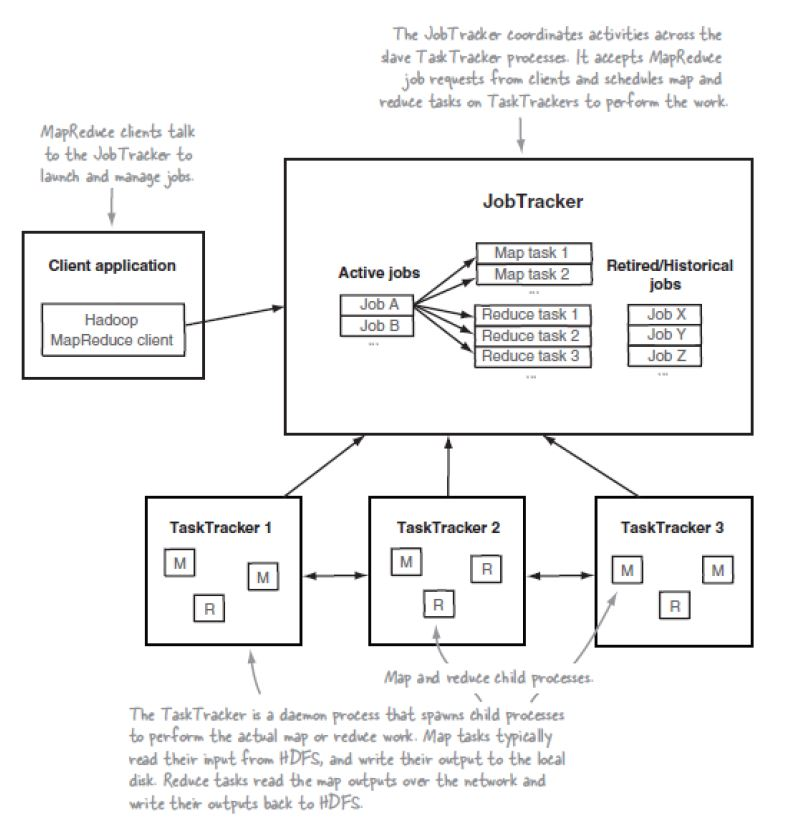
\includegraphics[scale=0.5]{mapreducearchitecture}  
		\caption[Gambar Arsitektur MapReduce]{Arsitektur MapReduce} 
		\label{fig:HDFS Architecture} 
		\end{figure}
		
	Komponen MapReduce pada master node menjalankan daemon JobTracker yang merupakan
	daemon yang menghubungkan proses pada Hadoop dengan aplikasi. JobTracker bertugas melakukan
	pemecahan pekerjaan yang dikirimkan klien menjadi unit-unit pekerjaan map dan reduce. Job-
	Tracker akan mendistribusikan unit-unit pekerjaan tersebut ke slave node, melakukan penjadwalan
	komputasi, dan melakukan pengawasan terhadap pemrosesan yang dilakukan dalam slave node.
	Komponen MapReduce pada setiap slave node menjalankan daemon TaskTracker yang bertugas
	untuk melakukan eksekusi pemrosesan di dalam slave node. TaskTracker akan selalu berkomunikasi
	dengan JobTracker untuk memantau jalannya proses. Jika komunikasi tersebut terputus, dapat
	diasumsikan proses pada TaskTracker tersebut gagal dan unit pekerjaan yang sesuai akan 					dikirimkan oleh JobTracker ke slave node lain yang terdapat di dalam klaster.
	
	MapReduce terdiri dari komponen-komponen mapper dan reducer. Pekerjaan yang dikirimkan
	ke dalam klaster akan dipecah menjadi pekerjaan map dan reduce yang berjalan secara paralel.
	Setiap node dalam map dan reduce dapat berdiri sendiri dan tidak tergantung pada node-node map
	atau reduce lainnya. Ketergantungan yang ada hanya ketergantungan node-node reduce terhadap
	node-node map. Pemrosesan ini dilakukan dengan model share-nothing, yaitu data yang diolah
	tidak dibagikan antarnode untuk mencegah node-node tersebut saling menunggu untuk memakai
	sumber daya. Implementasi aplikasi dengan MapReduce dapat dilakukan dengan mendefinisikan fungsi 	map dan reduce. Fungsi map menerima masukan berupa pasangan-pasangan key dan value dan 					memberikan keluaran berupa list key dan value. Fungsi reduce menerima masukan berupa key dan 			list value dan memberikan keluaran berupa pasangan key dan value.
	
		\begin{figure}[H] 
		\centering  
		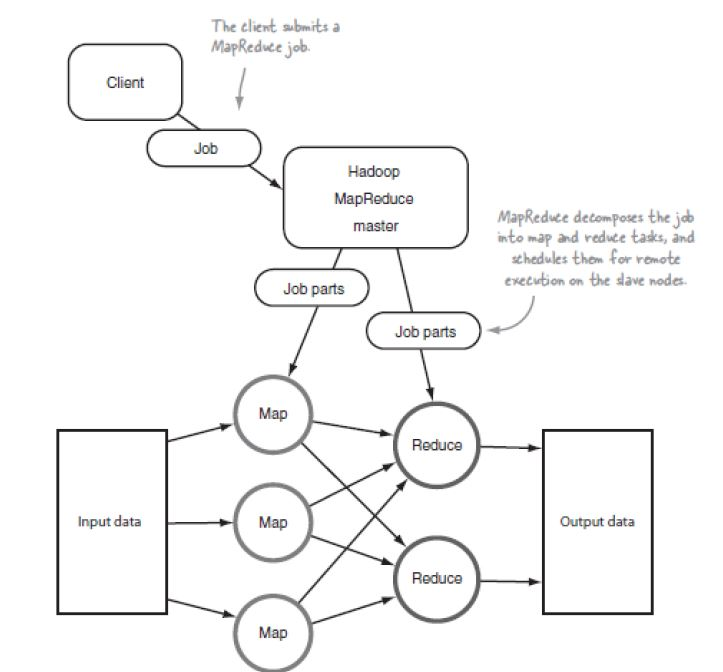
\includegraphics[scale=0.5]{MapReduceProses}  
		\caption[Gambar Proses MapReduce]{Proses MapReduce} 
		\label{fig:processing-events relationship} 
		\end{figure}
	
	Gambar 2.10 merupakan gambaran proses yang terjadi ketika klien mengirimkan sebuah pekerjaan
	MapReduce ke dalam klaster. Pekerjaan yang dikirimkan oleh klien dapat berupa file jar atau
	xml. Pekerjaan tersebut akan dipecah menjadi unit-unit pekerjaan map dan reduce oleh komponen
	MapReduce yang terdapat pada master node sebelum didistribusikan ke slave node.
	Data masukan akan diproses menggunakan komponen mapper pada MapReduce dan format
	data harus berupa pasangan key dan value. Untuk setiap pasang key dan value tersebut, dilakukan
	pemrosesan menggunakan fungsi map dan mengembalikan keluaran berupa list pasangan key dan
	value yang baru. Nilai key pada tahap pemrosesan ini pada umumnya tidak diperhitungkan.
	Hasil keluaran dari mapper akan diproses terlebih dahulu sebelum dijadikan masukan untuk
	komponen reducer. Tahap pemrosesan ini disebut sebagai tahap shuffle and sort. Setiap pasangan
	
	key dan value akan diurutkan berdasarkan key yang dimiliki dan mengelompokkan semua value yang
	mempunyai key yang sama untuk dimasukkan ke node reducer yang sama. Proses ini akan menjadi
	kompleks ketika semua key yang ada dalam list keluaran mempunyai nilai yang berbeda-beda.
	Komponen reducer menerima masukan yang berasal dari hasil pada tahap shuffle and sort yang
	berupa pasangan key dan list value. Untuk setiap nilai key yang ada, fungsi reduce pada reducer
	akan dipanggil satu kali dan memberikan keluaran berupa pasangan key dan value yang baru.
	Keluaran dari proses reduce tersebut dapat ditulis ke file yang berada di HDFS maupun ke dalam
	basis data.
	}
\end{itemize}
\label{sec:Hadoop}

\section{Scala}
Scala merupakan bahasa pemrograman fungsional dan berorientasi objek. Sebagai bahasa pemrograman
berorientasi objek, setiap sifat dan kemampuan objek Scala dideskripsikan dalam
kelas-kelas Scala. Sebagai bahasa pemrograman fungsional, penggunaan fungsi high-order dan
pendefinisian fungsi anonim dapat dilakukan pada Scala. Fungsi high-order merupakan fungsi yang
menerima fungsi lain sebagai parameter. Fungsi anonim merupakan fungsi yang didefinisikan tanpa
memerlukan nama fungsi dan hanya langkah-langkah yang dilakukan oleh fungsi tersebut.
Scala merupakan bahasa pemrograman yang berdasar pada Java Virtual Machine, sehingga
Scala dapat dikompilasi menjadi Java Byte Code dan dapat dijalankan pada Java Virtual Machine.
Oleh karena itu, Scala dapat beroperasi dengan baik bersamaan dengan Java. Library Scala dapat
digunakan pada aplikasi berbasis Java dan demikian pula sebaliknya.

\subsection{variable}
Scala mempunyai dua jenis variabel, yaitu variabel yang dapat diubah dan tidak dapat diubah.
Deklarasi variabel yang dapat diubah dilakukan dengan menggunakan kata kunci var, sedangkan
variabel yang tidak dapat diubah atau konstanta menggunakan kata kunci val. Pengubahan
nilai konstanta akan menyebabkan terjadinya error. Contoh deklarasi variabel dapat dilihat pada
potongan kode berikut.

\subsection{Fungsi}
Deklarasi fungsi pada Scala dapat dilakukan dengan menggunakan kata kunci def. Header dari fungsi
dapat dituliskan dengan format def \texttt{namaFungsi(namaParameter: TipeData): TipeKeluaran}.
\begin{lstlisting}[language=Scala, caption=Deklarasi Fungsi]
def add( firstInput : Int , secondInput : Int): Int = {
  val sum = firstInput + secondInput
  return sum
  }
\end{lstlisting}
Bahasa pemrograman Scala mempunyai filosofi kode yang ringkas, sehingga deklarasi fungsi
dapat diringkas lebih lanjut. Jika suatu fungsi menggunakan sebuah variabel sebagai penampung
hasil komputasi singkat, maka penulisan deklarasi tersebut dapat diringkas menjadi seperti deklarasi
sebuah variabel. Penulisan deklarasi tersebut dapat diringkas menjadi seperti berikut ini.

\begin{lstlisting}[language=Scala, caption=Deklarasi Fungsi Ringkas]
def add( firstInput : Int , secondInput : Int) = firstInput +
secondInput
\end{lstlisting}


\subsubsection{Fungsi Lokal}
Sebuah fungsi dapat didefinisikan di dalam sebuah fungsi lain. Fungsi yang didefinisikan di dalam
fungsi lain tersebut disebut dengan fungsi lokal. Fungsi lokal tersebut dapat mengakses semua
variabel yang ada pada fungsi tempat fungsi lokal tersebut didefinisikan, tetapi fungsi lokal tersebut hanya dapat diakses oleh fungsi yang mendefinisikan fungsi lokal tersebut.

\subsubsection{Fungsi Highorder}
Fungsi yang menerima fungsi lain sebagai parameter disebut dengan fungsi high-order. Fungsi
high-order tersebut dapat membantu mengurangi duplikasi pada kode program dan membuat kode
yang lebih ringkas.

\begin{lstlisting}[language=Scala, caption=Contoh fungsi \textit{high-order}]
def encode (n: Int , f: (Int) => Long ): Long = {
  val x = n * 10
  f(x)
  }
\end{lstlisting}

\subsubsection{Fungsi Anonim}
Selain menggunakan cara-cara yang sudah dijabarkan sebelumnya, fungsi Scala dapat dideklarasikan
dengan menggunakan hanya parameter fungsi dan langkah-langkah yang perlu dilakukan dalam
fungsi. Fungsi yang dideklarasikan dengan cara tersebut dapat dijadikan sebagai masukan dari
sebuah fungsi high-order atau dimasukkan sebagai nilai dari variabel. Fungsi yang dideklarasikan
dengan cara seperti ini disebut dengan fungsi anonim.
\begin{lstlisting}[language=Scala, caption=Contoh fungsi anonim]
(x: Int) => {
	x + 100
}
\end{lstlisting}

Bagian kiri dari karakter panah merupakan parameter dari fungsi, sedangkan bagian kanan
merupakan isi fungsi atau operasi yang dilakukan oleh fungsi. Isi fungsi tersebut dimasukkan ke
dalam tanda kurung kurawal.
Jika fungsi tersebut hanya berisi satu baris perintah saja, maka penulisan isi fungsi tidak
memerlukan kurung kurawal. Penulisan fungsi tanpa kurung kurawal tersebut dapat diringkas
menjadi seperti berikut ini.

\begin{lstlisting}[language=Scala, caption=Penulisan ringkas fungsi anonim]
(x: Int) => x + 100
\end{lstlisting}

Fungsi anonim tersebut dapat digunakan sebagai masukan dari fungsi high-order encode yang
sudah didefinisikan sebelumnya.

\begin{lstlisting}[language=Scala, caption=Penggunaan fungsi anonim pada fungsi \textit{high-order}]
val code = encode (10 , (x: Int) => x + 100)
\end{lstlisting}


\subsection{Kelas}
Kelas merupakan sebuah konsep pemrograman berbasis objek. Pada tingkat dasar, penggunaan
kelas merupakan sebuah teknik penyusunan kode untuk mengelompokkan data dan operasioperasinya.
Secara konsep, kelas merepresentasikan sebuah entitas dengan sifat-sifat dan kemampuankemampuannnya.
Kelas pada Scala mempunyai kemiripan seperti kelas pada bahasa pemrograman berorientasi
objek yang lain. Kelas terdiri dari sejumlah field dan method dengan field adalah variabel yang
menyimpan data dan method menyimpan kode yang dapat dieksekusi. Method merupakan fungsi

yang didefinisikan di dalam kelas dan mempunyai akses pada semua variabel yang ada pada kelas
tersebut.
Sebuah kelas merupakan cetakan untuk membuat objek pada saat runtime. Kelas didefinisikan
pada kode sumber, sedangkan objek didefinisikan pada saat runtime. Sebuah kelas didefinisikan
dengan kata kunci class, diikuti dengan nama kelas, sejumlah parameter kelas yang dimasukkan
ke dalam sebuah kurung, dan field beserta method yang dimasukkan ke dalam kurung kurawal.

\begin{lstlisting}[language=Scala, caption=Contoh definisi kelas]
class Car(mk: String , ml: String , cr: String ){
  val make = mk
  val model = ml
  val color = cr
 
  def repaint ( newColor : String ) = {
  color = newColor
  }
}
\end{lstlisting}

Berdasarkan definisi kelas di atas, instansi dari kelas tersebut dapat dibuat dengan kata kunci
new.

\begin{lstlisting}[language=Scala, caption=Pembuatan instansi kelas]
	val mustang = new Car("Ford", "Mustang", "Red")
	val corvette = new Car("GM", "Corvette", "Black")
\end{lstlisting}

Pada umumnya, sebuah kelas digunakan sebagai struktur data yang mutable atau dapat diubah.
Setiap objek yang menjadi instansi sebuah kelas mempunyai state yang dapat berubah-ubah. Oleh
karena itu, sebuah kelas dapat mempunyai field yang didefinisikan dengan menggunakan kata kunci
var. Penghapusan objek-objek yang sudah dibuat tidak perlu ditangani karena Scala berjalan pada
JVM dan garbage collector Java sudah mengatasi hal tersebut.\newline

\subsubsection{\textit{Singleton}}
Terkait dengan penggunaan struktur kelas, salah satu pola perancangan yang ada pada pemrograman
berorientasi objek adalah penggunaan kelas yang hanya dapat diinstansiasi sebanyak satu kali saja.
Kelas yang mempunyai sifat tersebut adalah singleton. Definisi kelas singleton pada Scala dilakukan
dengan menggunakan kata kunci \texttt{object}.
\begin{lstlisting}[language=Scala, caption=Contoh definisi kelas singleton]
	object DatabaseConnection {
	def open ( name : String ): Int = {
	// isi method open ()
	}
	
	def read ( streamId : Int): Array [ Byte ] = {
	isi method read ()
	}

	def close (): Unit = {
	// isi method close ()
		}
	}
\end{lstlisting}

\subsubsection{Case Class}
Sebuah kelas yang didefinisikan dengan kata kunci class akan bersifat mutable. Case class
merupakan kelas yang didefinisikan dengan penambahan kata kunci case.
\begin{lstlisting}[language=Scala, caption=Definisi \textit{case class}]
case class Message ( from : String , to: String , content : String )
\end{lstlisting}

Penggunan kata kunci tersebut memberikan beberapa keuntungan, seperti pembuatan method
yang memiliki nama sama dengan nama kelas tersebut. Hal ini memungkinkan pembuatan instansi
case class tanpa menggunakan kata kunci new.
\begin{lstlisting}[language=Scala, caption=Pembuatan instansi \textit{case class}]
val request = Message ("harry", "sam", "fight")
\end{lstlisting}

Selain itu, semua parameter yang ada pada definisi kelas akan menjadi field kelas yang nonmutable
atau tidak dapat diubah. Sifat ini memungkinkan field kelas tersebut diakses dari luar kelas.
Definisi parameter tersebut dengan penggunaan kata kunci val pada setiap parameter. Penggunaan
case class juga memungkinkan akses pada tambahan method toString, hashCode, equals, dan
copy.

\subsection{Kelas option}
Kelas Option merupakan sebuah kelas yang digunakan sebagai tipe data keluaran fungsi. Kelas
ini dapat menangani keluaran fungsi yang dapat berupa sebuah nilai tertentu atau berupa null.
Masalah ini ditangani dengan dua kelas turunan dari Option, yaitu kelas Some dan kelas None.
Sebagai contoh, fungsi untuk mengubah tipe data String menjadi Int sebaiknya memiliki tipe
keluaran berupa Option dan bukan menggunakan tipe keluaran Int. Hal ini disebabkan nilai
String yang diberikan dapat berupa angka maupun angka yang bercampur dengan huruf. String
yang berupa angka bercampur huruf akan menimbulkan error jika digunakan sebagai masukan
fungsi pengubahan dengan tipe keluaran \texttt{Int}.
\begin{lstlisting}[language=Scala, caption= Fungsi pengubah \texttt{String} menjadi \texttt{Int}]
val request = Message ("harry", "sam", "fight")
\end{lstlisting}

Fungsi tersebut dapat menangani String masukan dengan format yang salah, yaitu dengan
mengeluarkan nilai berupa None. Jika masukan tersebut benar, maka nilai yang dikembalikan
tersebut adalah Some(angka).

\begin{lstlisting}[language=Scala, caption= Contoh pemanfaatan kelas Some dan None]
def toInt2 (str: String ): Option [Int] = {
  try {
  Some ( Integer . parseInt (str . trim ))
  }
  catch {
  case e: NumberFormatException => None
  }
  }
\end{lstlisting}

\subsection{Trait}
Trait merepresentasikan antarmuka yang didukung oleh hirarki kelas yang terhubung. Trait pada
Scala mempunyai kemiripan dengan interface pada Java. Akan tetapi, interface Java hanya
mempunyai nama, parameter, dan tipe keluaran method sedangkan trait Scala dapat mempunyai
implementasi dari method. Trait mempunyai kemiripan dengan kelas abstrak, hanya saja kelas
dapat diturunkan dari satu buah kelas tetapi dapat diturunkan dari beberapa trait.
\begin{lstlisting}[language=Scala, caption= Contoh penggunaan trait]
trait Shape {
  def area (): Int
  }
  
  class Square ( length : Int) extends Shape {
  def area = length * length
  }

  class Rectangle ( length : Int , width : Int) extends Shape {
  def area = length * width
  }
 
  val square = new Square (10)
\end{lstlisting}

\subsection{Tuple}
Pengembalian hasil dari sebuah fungsi hanya dapat berupa satu nilai saja, tetapi Scala mempunyai
struktur data yang dapat mengembalikan lebih dari satu nilai. Tuple merupakan salah satu
struktur data dalam Scala yang berupa wadah untuk menyimpan dua atau lebih elemen yang dapat
mempunyai tipe berbeda. Tuple bersifat immutable atau tidak dapat diubah setelah dibuat. Scala
menyediakan kelas-kelas untuk setiap tuple yang mempunyai 2 sampai 22 elemen, yaitu Tuple2,
Tuple3, sampai dengan Tuple22. Setiap elemen dapat diakses dengan menggunakan indeks.
\begin{lstlisting}[language=Scala, caption= Deklarasi dan penggunaan tuple]
	val tuple2 = ("Rod", 3)
	val tuple3 = ("10", "Wombat", true )
	println ( tuple2 _.1 + "has" + tuple2 _.2 + "coconuts")
\end{lstlisting}

\subsection{Koleksi}
Koleksi merupakan struktur data yang berupa tempat penyimpanan yang berisi nol atau lebih
elemen. Setiap jenis koleksi pada Scala mempunyai antarmuka yang sama, sehingga penguasaan
pada salah satu jenis koleksi dapat memudahkan penggunaan koleksi-koleksi Scala lainnya. Koleksi
pada Scala dapat dikelompokkan menjadi tiga kategori, yaitu sequence, set, dan map.\newline

\subsubsection{Sequence}
Sequence merupakan koleksi elemen dengan keterurutan tertentu. Oleh karena keterurutan tersebut,
setiap elemen dapat diakses melalui posisi elemen-elemen tersebut di dalam koleksi.
Array merupakan urutan elemen yang terindeks dengan tipe data yang sama. Struktur data
array merupakan struktur data yang bersifat mutable karena setiap elemen dalam array dapat
diubah. Panjang array bersifat tetap, sehingga tidak memungkinkan penambahan elemen baru
setelah array dibuat. Indeks pada array dimulai dari 0. Untuk mengambil nilai atau melakukan
perubahan pada sebuah elemen dalam array, indeks elemen tersebut perlu dicantumkan di dalam
tanda kurung.

\begin{lstlisting}[language=Scala, caption= Contoh penggunaan array]
	val arr = Array (10 , 20, 30, 40) // definisi array
	arr (0) = 50 // mengubah elemen indeks 0 menjadi 50
	val first = arr (0) // mengambil elemen indeks 0
\end{lstlisting}

List merupakan urutan elemen linier yang mempunyai tipe data yang sama. Berbeda dengan
array, list merupakan struktur data dengan nilai-nilai yang tidak bisa diubah. Elemen-elemen dari
sebuah list dapat diakses dengan menggunakan indeks, tetapi list bukan struktur data yang efisien
untuk melakukan akses data berdasarkan nomor indeks elemen. Hal ini disebabkan waktu akses
indeks sebanding dengan banyak elemen di dalam list.

\begin{lstlisting}[language=Scala, caption= Macam-macam cara pembuatan list]
	val xs = List (10 , 20, 30, 40)
	val ys = (1 to 100) . toList
	val zs = someArray . toList
\end{lstlisting}

Vector adalah kelas yang merupakan gabungan dari kelas list dan array. Kelas Vector menggabungkan
karakteristik kinerja dari kedua kelas tersebut dan waktu akses melalui indeks serta
waktu akses linier menjadi konstan. Selain itu, kelas Vector memungkinkan akses elemen secara
acak dan pengubahan elemen dengan cepat.


\begin{lstlisting}[language=Scala, caption= Contoh penggunaan Vector]
	val v1 = Vector (0, 10, 20, 30, 40)
	val v2 = v1 :+ 50
	val v3 = v2 :+ 60
	val v4 = v3 (4)
	val v5 = v3 (5)
\end{lstlisting}

\subsubsection{\textit{Set}}
Set merupakan sebuah koleksi yang terdiri dari elemen-elemen yang berbeda dan tidak terurut.
Set tidak menggunakan indeks, sehingga akses elemen berdasarkan indeks tidak dimungkinkan.
Set mendukung dua buah operasi dasar, yaitu contains untuk memeriksa apakah set tersebut
mempunyai elemen yang menjadi parameter dan isEmpty untuk memeriksa apakah set tersebut
kosong. Kedua operasi dasar tersebut akan mengembalikan hasil berupa true atau false.

\begin{lstlisting}[language=Scala, caption= Contoh deklarasi set]
	val fruits = Set("apple", "orange", "pear", "banana")
\end{lstlisting}

\subsubsection{\textit{Map}}
Map merupakan koleksi yang terdiri dari pasangan key-value. Map merupakan struktur data yang
efisien untuk melakukan akses suatu nilai dengan menggunakan kunci atau key. Pada bahasa-bahasa
lain, map dikenal dengan istilah kamus, associative array, atau hash map.

\begin{lstlisting}[language=Scala, caption= Contoh deklarasi dan penggunaan map]
	val capitals = Map("USA" -> "Washington D.C.", "UK" -> "London", 
					"India" -> "New Delhi")
	val indiaCapital = capitals ("India")
\end{lstlisting}

\subsection{Percabangan}
Percabangan atau ekspresi bersyarat mengarahkan jalannya program berdasarkan hasil dari evaluasi
syarat percobaan. Jika hasil tersebut mengembalikan nilai benar maka satu cabang kode akan
dijalankan, jika tidak maka cabang kode lain yang akan dijalankan.
\begin{lstlisting}[showstringspaces=false, language=Scala, caption= Contoh dasar percabangan]
	if ( inputNumber < 5)
		println ("Number is smaller than 5")
	else
		println ("Number is greater than or equal to 5")
\end{lstlisting}

Percabangan dengan cabang lebih dari dua cabang dapat dilakukan dengan menggunakan kata
kunci else if. Kata kunci tersebut dapat digunakan lebih dari satu kali dalam sebuah percabangan,
berbeda dengan penggunaan if dan else yang hanya dapat digunakan masing-masing satu kali
dalam sebuah percabangan pada tingkat yang sama. Selain itu, kode yang dijalankan pada
percabangan perlu dimasukkan ke dalam kurung kurawal jika kode tersebut lebih dari satu baris
pernyataan.

\begin{lstlisting}[showstringspaces=false, language=Scala, caption= Penggunaan else if dalam percabangan]
if (( executeFlag == true ) && ( firstNumber - secondNumber ) > 0) {
	positiveDiff = firstNumber - secondNumber
	println ("The positive difference : "+ positiveDiff )
} else if (( executeFlag == true ) && ( secondNumber - firstNumber ) > 0){
	positiveDiff = secondNumber - firstNumber
	println ("The positive difference : "+ positiveDiff )
} else if( executeFlag == true ) {
	println ("Two numbers are equal ")
} else {
	println ("The execution flag is not set")
}
\end{lstlisting}

\subsection{Pengulangan}
Pengulangan dapat dilakukan dengan menggunakan kata kunci for atau menggunakan \texttt{while}.

\textbf{Pengulangan dengan for}\newline
Pengulangan dengan menggunakan for merupakan pengulangan yang dikendalikan dengan menggunakan
dua buah variabel, yaitu variabel yang menyatakan titik mulai dan variabel yang menyatakan
titik akhir pengulangan.

\begin{lstlisting}[showstringspaces=false, language=Scala, caption= Contoh dasar penggunaan for]
	for(i <- 1 until 5)
		print (i+", ")
	// Keluaran : 1, 2, 3, 4
\end{lstlisting}

Selain itu, for dapat digunakan untuk melakukan iterasi pada sebuah array.

\begin{lstlisting}[showstringspaces=false, language=Scala, caption= Iterasi pada array]
	for(i <- (1 to 5).reverse)
		println (i+", ")
	// Keluaran : 5, 4, 3, 2, 1
\end{lstlisting}

Pengulangan dapat dilakukan untuk menampilkan angka secara terurut menurun tanpa menggunakan
array. Besarnya lompatan antara angka yang satu dengan yang lain dinyatakan dengan
menggunakan kata kunci \texttt{by}.

\begin{lstlisting}[showstringspaces=false, language=Scala, caption= Pengulangan angka secara terurut menurun]
	for(i <- 5 to 1 by -1)
		print (i+", ")
	// Keluaran : 5, 4, 3, 2, 1
\end{lstlisting}

Pengulangan dapat dilakukan secara bertingkat dengan menggunakan titik awal yang mempunyai
nama variabel berbeda. Setiap tingkatan tersebut dipisahkan dengan simbol titik koma (;) dan
pengulangan dimulai dari tingkatan yang berada pada bagian paling kanan.

\begin{lstlisting}[showstringspaces=false, language=Scala, caption= Pengulangan bertingkat]
	for(i <- 1 to 3; j <- 1 to 2)
		print (i+","+j+"; ")
	// Keluaran : 1 ,1; 1 ,2; 2 ,1; 2 ,2; 3 ,1; 3 ,2;
\end{lstlisting}

\textbf{Pengulangan dengan while}\newline
Pengulangan dengan menggunakan while memerlukan syarat pengulangan tersebut dihentikan
dan blok kode yang akan dijalankan selama pengulangan berlangsung. Jika hasil pemeriksaan
syarat tersebut mengembalikan nilai benar, maka blok kode yang ada di dalam kurung kurawal
akan dijalankan. Hal tersebut akan terus berulang sampai hasil pemeriksaan syarat tersebut
mengembalikan nilai salah.

\begin{lstlisting}[showstringspaces=false, language=Scala, caption= Pengulangan menggunakan while]
	while (i < inputNumber){
		if( inputNumber % i == 0){
		isPrime = false
	}
	i += 1
  }
\end{lstlisting}

Penggunaan while memungkinkan pengulangan dengan melakukan pemeriksaan syarat terlebih
dahulu kemudian menjalankan blok kode jika hasil pemeriksaan berhasil benar. Hal ini berbeda
dengan penggunaan do-while yang akan selalu menjalankan blok kode minimal satu kali sebelum
pengulangan dihentikan.

\begin{lstlisting}[language=Scala, caption= Penggunaan do-while]
	var i = 1
	do {
		print (i+",")
		i += 1
	} while (i < 5)
\end{lstlisting}


\subsection{Operasi Baca Tulis File}
Membaca Data dari FileOperasi membaca data dari sebuah file pada Scala menggunakan library yang disediakan oleh Java. Scala hanya menyediakan library untuk mereferensikan alamat dari file yang akan dibaca dengan menggunakan kelas \texttt{Source}.
\begin{lstlisting}[showstringspaces=false, language=Scala, caption= Membaca file teks]
import java .io .{ IOException , FileNotFoundException }
import scala .io. Source

object ReadFromTextFile {
def main ( args : Array [ String ]): Unit = {
val fileName = "/Users/.../temp/InputFile.txt"
var source :scala.io.BufferedSource = null
try {
	source = Source.fromFile(fileName)
	for (line <- source.getLines()){
	println (line)}
	} catch {
	case e: FileNotFoundException => println ("File not found.")
	case e: IOException => println ("IO problem .")
	case e: Exception => println (" Something went wrong .")
	} finally {
	source.close ()
		}
	}
}
\end{lstlisting}

\textbf{Menulis Data pada File}\newline
Seperti halnya pada operasi membaca file, operasi menulis file juga dilakukan dengan menggunakan
library yang disediakan oleh Java.
\begin{lstlisting}[showstringspaces=false,language=Scala, caption= Menulis file teks]
import java .io .{ File , PrintWriter }
object WriteToFile {
	def main ( args : Array [ String ]):Unit = {
	val outFileName = "/Users/.../temp/OutputFile .txt"
	var printWriter : PrintWriter = null
	try {
		printWriter = new PrintWriter (new File(outFileName))
		printWriter.write("Scala is purely OO language.")
	} catch {
		case e: Exception => println ("Something went wrong.")
	} finally {
		printWriter . close ()
	}
  }
}
}
\end{lstlisting}


\section{Sistem Terdistribusi Spark}
\textit{Apache Spark} merupakan \textit{platform} komputasi klaster yang dirancang untuk berjalan dengan cepat ketika mengolah data yang sangat besar dan untuk tujuan penggunaan umum. \textit{Spark} merupakan penerus dari model pemprosesan \textit{MapReduce} pada \textit{Hadoop} dengan jenis komputasi lebih banyak yang dapat dilakukan. Salah satu fitur utama yang ditawarkan \textit{Spark} untuk kecepatan adalah kemampuan untuk menjalankan komputasi di memori. Namun, sistem ini lebih efisien dari MapReduce untuk aplikasi kompleks yang berjalan pada disk karena \textit{Spark} menggunakan DAG(\textit{Directed Acyclic Graph}) \textit{Engine} yang mengoptimasi workflow. DAG bekerja dengan cara  menentukan jenis suatu flow yang akan memproses data yang masuk. \textit{Spark} akan mencari cara pengerjaan mana yang paling optimal untuk melakukan pendekatan bagi masalah ini secara keseluruhan. \textit{Spark} juga akan mengoptimasi \textit{workflow} dari pengerjaan tersebut. \textit{Spark} lebih bisa beradaptasi dengan pengerjaan pemrosesan data secara menyeluruh karena itu spark bisa bekerja dengan cepat.

\textit{Spark} telah dioptimalkan untuk berjalan pada memori sehingga mempercepat pengolahaan data dibandingkan dengan pendekatan alternatif lain seperti MapReduce pada hadoop yang menulis dan membaca data secara langsung pada \textit{hard drive} komputer pada setiap tahap pemrosesan. Dengan demikian kecepatan pengolahaan data menggunakan spark dapat menjadi lebih cepat dibandingkan dengan Hadoop. 

\textit{Spark} sering digunakan dalam pemanggilan kueri interaktif pada set data yang besar, pengolahaan data streaming dari sensor maupun sistem finansial, dan tugas-tugas pembelajaran mesin. Selain itu, pengembangan juga dapat menggunakan spark untuk tugas-tuga pemrosesan data lainnya dengan memanfaatkan \textit{library} pengembang dan API serta dukungan untuk bahasa pemrograman java, Python, R, dan Scala. Spark biasa digunakan bersama dengan HDFS(\textit{Hadoop distributed File System}) sebagai pengganti media penyimpanan. \textit{Spark} mempunyai lima buah fitur kunci, yaitu; \textit{easy to use, fast, general purpose, scalable}, dan \textit{falut tolerant}.
\begin{enumerate}
	\item{\textit{Easy to Use} \newline
	Spark menyediakan lebih dari 80 jenis operator untuk melakukan proses pengolahan data. 			
	Sehingga pengolahaan data yang lebih kompleks bisa dilakukan dengan mudah.
	}
	
	\item{\textit{Fast} \newline
	\textit{Spark} meminimalisir akses data pada disk dengan menyimpan data pada 					
	\textit{cache}. Sehingga pengolahaan data menggunakan set data yang sama hanya memerlukan 		
	akses pada disk sebanyak satu kali.
	}
	
	\item{\textit{General Purpose} \newline
	\textit{Spark} sudah mempunyai \textit{library} sendiri untuk melakukan \textit{batch 			
	processing}, analisis interaktif pada pengolahan \textit{data stream}, pembelajaran mesin dan 
	komputasi graf. Setiap mesin tersebut tidak memerlukan mesin klaster tersendiri untuk 		
	melakukan jenis pengolahan tertentu sehingga mengurangi kompleksitas operasional dan 			
	menghindari duplikasi kode maupun data.
	}
	
	\item{\textit{Scalability} \newline
	Sama seperti pada Hadoop, peningkatan kapasitas pengolahan data dapat dilakukan dengan 			
	menambahkan mesin ke dalam klaster. Selain itu, penambahan mesin pada Spark memengaruhi 		
	kode aplikasi yang sudah ada.
	}
	
	\item{\textit{Fault Tolerant} \newline
	Kerusakan pada salah satu mesin pada klaster sudah ditangani oleh spark. Tetapi, perlu ada 		
	kode untuk menangani hal tersebut walaupun kerusakan tersebut tidak memengaruhi kinerja 		
	aplikasi.	
	}
	
\end{enumerate}
\subsection{Susunan Spark}
Sebuah proyek Spark mempunyai beberapa komponen yang terintegrasi dalam Spark Pada intinya, Spark adalah sebuah mesin komputasi yang bertugas untuk mendistribusikan dan memantau aplikasi yang terdiri dari banyak tugas komputasi yang tersebar  ke mesin pekerja atau klaster komputasi. Mesin inti Spark yang dapat berjalan cepat dengan tujuan penggunaan umum memberikan kekuatan tambahan untuk komponen dengan tingkatan yang tingkatan pada susunan yang dikhususkan untuk beban kerja yang beragam. Komponen-komponen ini dirancang untuk beroperasi dengan erat dan dapat digunakan dengan memanggil komponen ini sebagai library di dalam sebuah proyek perangkat lunak.

	\begin{figure}[H] 
	\centering  
	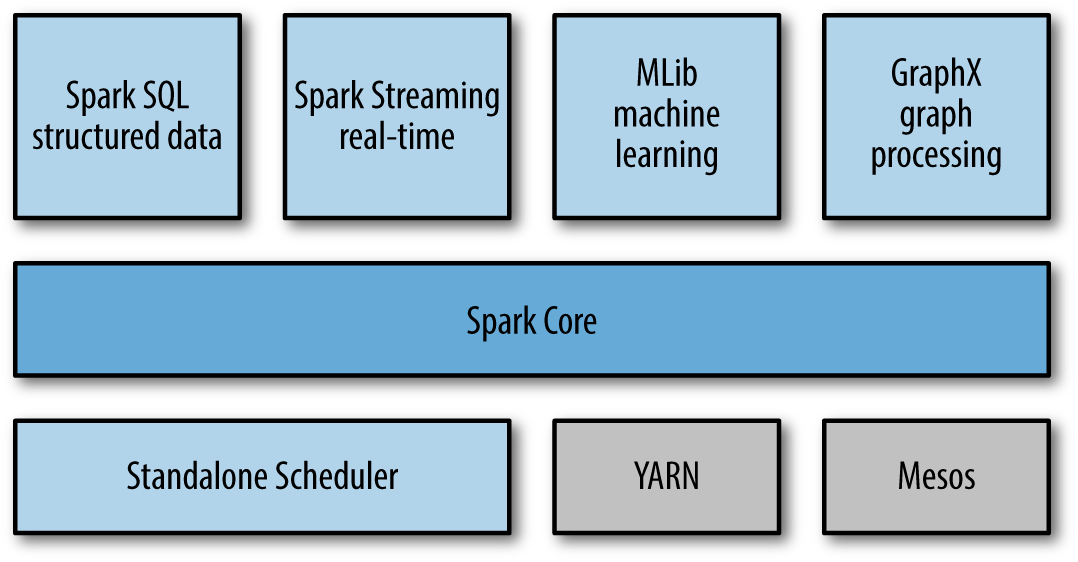
\includegraphics[scale=1]{spark-core}  
	\caption[Gambar { \it Spark unified stack}]{{\it Susunan Spark}} 
	\label{fig:processing-events relationship} 
	\end{figure}
	
Integrasi antar komponen yang erat tersebut memberikan beberapa keuntungan. Peratama \textit{library} di komponen-komponen tingkat tinggi akan mendapatkan keuntungan dari..
pada komponen-komponen ditingkat rendah. Kedua, beban untuk menjalankan susunan.. diminimalisir

\begin{itemize}
	\item[]{\textit{Spark Core}\newline
	\textit{Spark Core} merupakan fungsi dasar dari \textit{Spark} dan mempunyai komponen-			
	komponen untuk penjadwalan tugas, pengelolaan memori, pemulihan kegagalan, berinteraksi 		
	dengan sistem penyimpanan, dan lainnya. \textit{Spark Core} juga mempunyai API untuk 			
	mendefinisikan \textit{Resilient Distributed Dataset}(RDD) serta Spark Context akan dibahas 	
	lanjut pada 2.4.2
	}
	
	\item[]{\textit{Spark SQL}\newline
	Modul yang bekerja dengan data terstruktur menggunakan Hive yang memungkinkan programmer 		
	untuk menggabungkan SQL dengan bahasa pemrogramman spark seperti \textit{python, scala, dan 	
	java}.
	}
	
	\item[]{\textit{Spark Streaming}\newline
	API yang menyediakan pemrosesan data secara \textit{real-time}.komponen-komponen 				
	dari \textit{Spark Streming} hampir sama dengan \textit{Spark Core}. Seperti pengeloaan 		
	memori, pemulihan kegagalan, dan skalabilitas. \textit{Spark Streaming} mempunyai abstraksi 	
	dan API berupa \textit{Dstream} dan \textit{Streaming Context}. Spark Streaming akan 			
	dibahas lanjut pada 2.4.3
	}
	
	\item[]{\textit{Mlib}\newline
	Sebuah \textit{library} untuk \textit{machine learning}yang menyediakan beberapa tipe 			
	algoritma pembelajaran mesin yang dirancang untuk bekerja lintas klaster.
	}
	
	\item[] API untuk pemrosesan \textit{graph} dan komputasi \textit{graph-parallel}.
	
	\item[]{\textit{Cluster Manager}\newline
	Spark Dirancang untuk tetap efisien dalam peningkatan mesin dari satu hingga ribuan mesin. 		
	Untuk mencapai efisiensi tersebut sekaligus memaksimalkan fleksibilitas. Spark dapat 			
	menjalankan \textit{cluster manager} termasuk Hadoop dan YARN, Apache Mesos, dan 				
	\textit{Cluster Manager} yang sudah termasuk dalam spark yaitu Standalone Scheduler.
	}
\end{itemize}

\subsection{Application Programming Interface (API) Spark}
Kemampuan komputasi pada aplikasi spark ada dalam bentuk \textit{library}. \textit{library} tersebut ditulis dalam bahasa scala. Tetapi, menyediakan \textit{Applicataion Programming Interface} atau API dalam berbagai bahasa. Spark API mempunyai dua abstraksi penting, yaitu \textit{Spark Context} dan \textit{Resilient Distributed Datasets}(RDD). Kedua Abstraksi ini memungkinkan sebuah aplikasi untuk berinteraksi dengan Spark, terhubung dengan klaster, dan menggunakan sumber daya dalam \textit{Cluster}.

\subsubsection{Spark Context}
Spark Context Merupakan sebuah kelas yang didefinisikan dalam \textit{library Spark}. Spark Context merepresentasikan sebuah koneksi ke cluster spark dan diperlukan untuk membuat objek-objek lain yang disediakan oleh \textit{Spark} API. Sebuah aplikasi harus mempunyai objek \textit{Spark Context} yang aktif. Objek \textit{Spark Context} tersebut harus mempunyai konfigurasi untuk alamat spark master dan nama aplikasi. Spark Master merupakan cara SparkContext terkoneksi dengan klaster. Penggunaan kata kunci lokal menjalankan Spark dengan menggunakan sebuah thread pada satu mesin saja. Penggunaan thread tersebut dapat dikonfigurasi menjadi local$[n]$ untuk n buah thread atau local$[*]$ untuk menggunakan thread sejumlah core.

\subsubsection{Resilient Distributed Dataset(RDD)}
RDD adalah abstraksi dasar untuk merepresentasikan kumpulan objek yang dapat didistribusikan pada mesin-mesin dalam sebuah klaster. RDD dapat dibuat dengan menggunakan data yang bersumber dari luar seperti file dalam HDFS, tabel basis data, atau kumpulan objek local dan hasil transformasi yang dilakukan pada RDD yang sudah ada. Pembuatan RDD dengan data dari sumber luar memerlukan objek \textit{spark context}. karakteristik RDD.

\begin{enumerate}
	\item{\textit{Immutable}\newline
		RDD merupakan sebuah struktur data yang permanen. RDD yang dibuat tidak dapat 					
		dimodifikasi lebih lanjut. Sehingga operasi yang mengubah RDD akan mengembalikan RDD 			
		yang baru.
	}
	
	\item{\textit{Partitioned}\newline
	Data yang direpresentasikan oleh RDD terbagi menjadi partisi-partisi yang 						
	didistribusikan pada klaster mesin-mesin. Akan tetapi, partisi-partisi tersebut akan 			
	berada pada sebuah mesin yang sama jika \textit{Spark} hanya berjalan pada satu mesin 			
	saja. Di antara partisi RDD dengan partisi fisik set data terdapat pemetaan. Jenis 				
	Pemetaan tergantung pada sumber data seperti, blok-blok data HDFS mempunyai pemetaan 			
	satu ke satu dengan partisi-partisi RDD dan berapa partisi-partisi RDD dan beberapa 			
	partisi \textit{cassandra} dipetakan ke satu buah partisi RDD.
	}
	
	\item{\textit{Fault Tolerant}\newline
	RDD mengatasi kegagalan dari mesin klaster secara otomatis. Partisi RDD yang hilang 			
	pada mesin yang rusak tersebut akan dibuat ulang pada mesin lain. Hal ini dapat 				
	dilakukan karena spark menyimpan informasi keterhubungan antara RDD dan informasi 				
	tersebut digunakan untuk memulihkan bagian atau keseluruhan RDD yang hilang.
	}
	
	\item{\textit{Interface}\newline
	RDD merupakan sebuah antar muka untuk pemrosesan data yang didefinisikan sebagai kelas 			
	abstrak dalam \textit{library Spark}. RDD menyediakan antarmuka yang seragam untuk 				
	pemrosesan data yang berasal dari berbagai sumber. Selain itu RDD juga menyediakan kelas-		
	kelas implementasi konkret untuk sumber data yang berbeda.	
	}
	
	\item{\textit{Strongly typed}\newline
	Definisi kelas RDD mempunyai parameter tipe yang memungkinkan RDD untuk 						
	merepresentasikan data dengan tipe berbeda. RDD merupakan kumpulan elemen homogen yang 			
	terdistribusi dan elemen-elemen tersebut dapat bertipe \textit{Integer, Long, Float,String}, 
	atau tipe yang didefinisikan oleh pengembang aplikasi.
	}
	
	\item{\textit{In Memory}\newline
	Kelas RDD menyediakan API untuk komputasi klaster dalam memori. \textit{Spark} 			
	memungkinkan RDD untuk di-cache atau dipertahankan dalam memori. Operasi pada RDD yang 			
	ada dalam cache berjalan lebih cepat dibandingkan dengan operasi pada RDD yang tidak 			
	berada dalam cache.
	}
\end{enumerate}

\subsubsection{Transformasi dan Aksi}
Data yang sudah direpresentasikan dalam RDD dapat dioperasikan dengan menggunakan dua jenis operasi dasar, yaitu transformasi dan aksi.
\begin{enumerate}
	\item{\textit{transformasi}\newline
	RDD yang menjadi masukan dari sebuah operasi transformasi akan mengalami perubahan struktur 	
	atau nilai yang ada pada RDD. karena RDD bersifat \textit{immutable}, maka perubahan dari 		
	operasi ini secara konseptual akan dikembalikan dalam bentuk RDD baru.
	}
	
	\item{\textit{Aksi}\newline
	Operasi menjadi titik awal dari komputasi-komputasi yang telah terjadi pada RDD masukan. 		
	Pemanggilan operasi aksi akan memulai pembentukan RDD yang diperlakukan untuk komputasi. 		
	Operasi ini menerima masukan berupa RDD dan meberikan hasil berupa sebuah nilai.
	}
Operasi yang dilakukan pada RDD bersifat \textit{lazy} yang berarti operasi tersebut tidak akan dieksekusi oleh spark sampai ada operasi aksi. Evaluasi \textit{lazy} berarti ketika ada pemanggilan operasi transformasi pada RDD. Operasi tersebut tidak langsung dilakukan spark mencatat metadata untuk menandakan bahwa operasi tersebut sudah pernah diminta. Dengan demikian, RDD dapat disebut sebagai kumpulan instruksi untuk melakukan komputasi data yang dibuat dari kumpulan operasi transformasi.

\end{enumerate}
\subsection{Arsitektur Apache Spark}

	\begin{figure}[H] 
	\centering  
	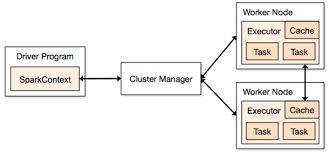
\includegraphics[scale=0.7]{spark-arsitektur}  
	\caption[Gambar Arsitektur {\it Spark}]{Arsitektur {\it Spark}} 
	\label{fig:processing-events relationship} 
	\end{figure}
	
Berdasarkan pada gambar sebuah aplikasi melibatkan lima entitas penting yaitu; driver program, cluster manager, worker, executor, dan task.
\begin{enumerate}
	\item{\textit{Driver Program}\newline
	Driver Program merupakan bagian dari aplikasi yang memulai menjalankan proses pengolahan 		data yang akan dilakukan. Driver program terhubung dengan komponen-komponen lain melalui 		objek \textit{Spark Context} yang terdapat dalam komponen ini. Objek \textit{Spark Context}
	akan melakukan koneksi dengan \textit{cluster manager}. Setiap klaster hanya akan mempunyai 	satu buah driver program atau satu buah objek spark context. 
	}
	
	\item{\textit{Cluster Manager}\newline
	\textit{Cluster Manager} berfungsi untuk mengelola sumber daya yang digunakan untuk proses 		pengolahan. Spark Context pada komponen driver program dapat terhubung dengan salah satu 		dari jenis-jenis cluster manager yang didukung oleh Spark, yaitu \textit{cluster manager} 		seperti \textit{Apache mesos} dan \textit{Yarn}. Setiap Cluster hanya memiliki satu buah 		\textit{cluster manager}.
	
	\item{\textit{Worker}\newline
	Worker merupakan komponen yang menyediakan unit pemrosesan dan alokasi memori untuk 			menyimpan sumber daya yang digunakan dalam proses yang berjalan. Setiap klaster dapat 			memiliki lebih dari satu buah worker dan setiap worker tersebut akan menjalankan aplikasi 		sebagai proses yang terdistribusi pada sebuah klaster.
	}
	
	\item{\textit{Executor}\newline
	\textit{Executor} merupakan proses yang dibuat oleh \textit{spark} pada setiap node worker 		untuk menjalankan aplikasi. \textit{Executor} yang terdapat pada setiap worker hanya dapat 		menangani proses untuk sebuah aplikasi saja, sehingga aplikasi yang berbeda akan mempunyai 		eksekutor yang berbeda. Setiap eksekutor mempunyai lama hidup yang sama dengan aplikasi 		sehingga akan berhenti ketiak aplikasi berhenti berjalan. Setiap Klaster dapat mempunyai 		lebih dari satu eksekutor dan jumlah tergantung pada banyak aplikasi.
	}
	
	\item{\textit{Task}\newline
	\textit{Task} merupakan unit pekerjaan terkecil yang dikirimkan ke executor. Unit pekerjaan 	tersebut akan dijalankan pada sejumlah \textit{thread} yang terdapat pada executor. Banyak 
	\textit{Thread} yang digunakan berbanding lurus dengan banyak partisi data yang diolah.
	}
		
	}
\end{enumerate}


\subsection{Spark Streaming}
\textit{Spark Streaming} adalah ekstensi dari API \textit{Spark Core} yang menyediakan pemprosesan \textit{Data Stream} yang bisa ditingkatkan performanya dengan menambah \textit{hardware baru}, bisa memproses data dengan banyak dan cepat, dan sistem masih bisa beroperasi ketika terjadi kegagalan. Data bisa dikumpulkan dari berbagai sumber seperti \textit{Kafka, Flume, Kinesis, atau TCP Socket}. Data yang terkumpul akan langsung diproses dengan algoritma yang kompleks seperti \textit{Map, Reduce, Join} dan \textit{Windowing}. Terakhir data yang telah diproses langsung dikirim ke \textit{File Systems, database} dan \textit{live dashboard}. Penjelasan lebih jelas ada pada gambar 2.12 berikut:

\begin{figure}[H] 
	\centering  
	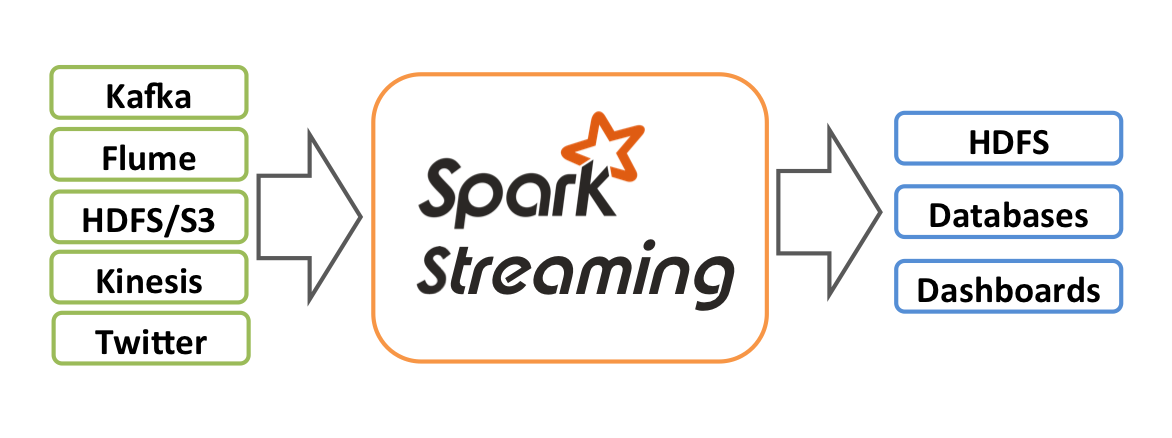
\includegraphics[scale=0.7]{streaming-arch}  
	\caption[Gambar Arsitektur {\it Spark Streaming}]{Arsitektur {\it Spark Streaming}} 
	\label{fig:processing-events relationship} 
	\end{figure}

\subsubsection{Arsitektur Spark Streaming}
\textit{Spark Streaming} bekerja dengan cara menerima input \textit{data streams}secara langsung dan membagai data tersebut menjadi beberapa potongan-potongan(\textit{batches}), yang nanti akan diproses oleh mesin \textit{Spark} untuk menghasilkan \textit{stream} akhir pada \textit{batches}. \textit{Spark Streaming} tidak memproses data secara periodik, hanya memproses yang duluan datang dan memutakhirkan hasil dari \textit{Spark Streaming} dari waktu ke waktu. Data langsung bisa dianalisis ketika datang dengan mengelompokannya ke beberapa bagian kecil dan langsung melakukan agregasi pada potongan data tersebut.

\begin{figure}[H] 
	\centering  
	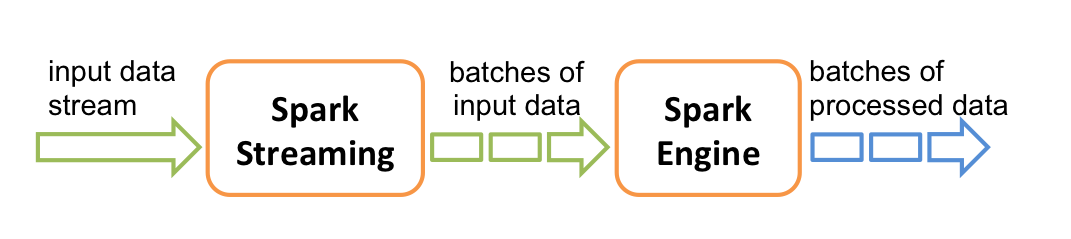
\includegraphics[scale=0.7]{streaming-flow}  
	\caption[Gambar Arsitektur {\it Spark Streaming}]{Arsitektur {\it Spark Streaming}} 
	\label{fig:processing-events relationship} 
	\end{figure}
	
	
Berdasarkan gambar 2.13 \textit{Data Streams} yang masuk akan diterima oleh \textit{reciever} lalu potongan-potongan data yang masuk pada selang waktu tertentu akan dihasilkan secara terus menerus dengan kata lain proses transformasi akan terus berlangsung ketika program dihentikan.
Lalu data yang telah dihasilkan dapat dikirimkan langsung ke \textit{external database} dengan data yang telah diagregasi sebelumnya.

transformasi dan aksi pada RDD bisa terjadi secara pararel pada node \textit{worker}. Artinya, proses RDD dibagi menjadi potongan kecil dan didistribusikan, potongan yang berbeda akan dikirim ke node yang berbeda. Potongan RDD tersebut akan didistribusikan ke seluruh klaster.

Aplikasi \textit{Spark Streaming} membutuhkan pengaturan tambahan untuk beroperasi tanpa henti. Aturan yang dimaksud adalah \textit{checkpointing} yang merupakan mekanisme utama pada \textit{Spark Streaming}. \textit{Checkpointing} memungkinkan penyimpanan data pada \textit{file system} seperti HDFS dan yang membuat \textit{Spark Streaming} menjadi \textit{fault tolerant}

\subsubsection{Abstraksi Spark Streaming}

Abstraksi dasar yang disediakan oleh \textit{Spark Streaming} disebut \textit{Discretized Streams} (\textit{DStreams}). \textit{Dstream} merupakan seluruh alur data yang datang dari \textit{recievers} Setiap Dstream dibuat pada potonga-potongan RDD yang merepresentasikan aliran data yang kontinu. Dstream memiliki dua buah operasi; transformasi dan \textit{output operation}. Transformasi bertugas untuk menghasilkan Dstream baru dan \textit{Output operation} bertugas untuk menuliskan data ke sistem eksternal. \textit{Dstream} menyediakan operasi yang hampir sama dengan operasi RDD dan mempunyai operasi sendiri yang digunakan untuk mengatur waktu seperti \textit{sliding window}.
 
setiap RDD yang ada pada Dstream mempunyai data dari interval tertentu yang akan ditunjukan pada gambar 2.14

\begin{figure}[H] 
	\centering  
	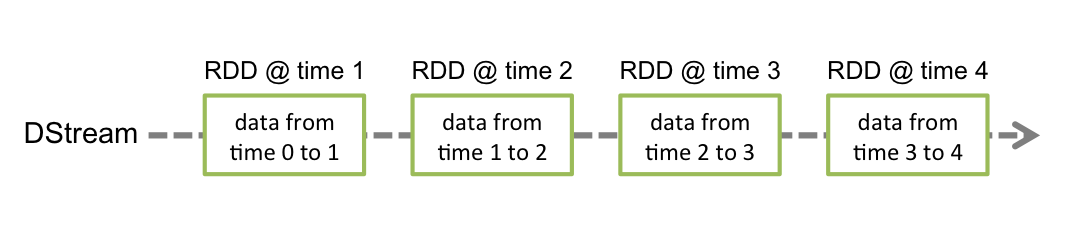
\includegraphics[scale=0.7]{streaming-dstream}  
	\caption[Gambar Alur {\it Dstream}]{Alur {\it Dstream}} 
	\label{fig:processing-events relationship} 
	\end{figure}

Pada setiap awal interval, \textit{batch} baru selalu dibuat dan setiap data yang muncul pada interval tersebut akan dimasukan ke \textit{batch} tersebut. Saat interval berakhir \textit{batch} telah selesai berkembang. Ukuran dari suatu interval ditentukan oleh sebuah parameter yang disebut \textit{batch interval}. Biasanya, ukurandari interval berkisar antara 500 milidetik sampai beberapa detik. Setiap input yang ada di dalam batch membentuk RDD dan diproses menggunakan \textit{Spark Jobs} untuk membuat RDD lain. RDD akan terus dibuat dan ditransformasi terus menerus sampai ada aksi yang memberhentikan \textit{Dstream}. Hasil dari transformasi \textit{Dstream} akan langsung dikirimkan ke sistem eksternal dalam bentuk \textit{batch}.\newline \textit{Dstream} merupakan salah satu abstraksi yang paling memudahkan pada spark streaming karena transformasi langsung diterapkan ke \textit{Dstream} bukan masing-masing RDD. Jadi, jika melakukan transformasi pada Dstream seluruh potongan RDD akan ikut bertransformasi. Namun, masing-masing RDD masih bisa diakses melalui \textit{Dstream}.

\begin{figure}[H] 
	\centering  
	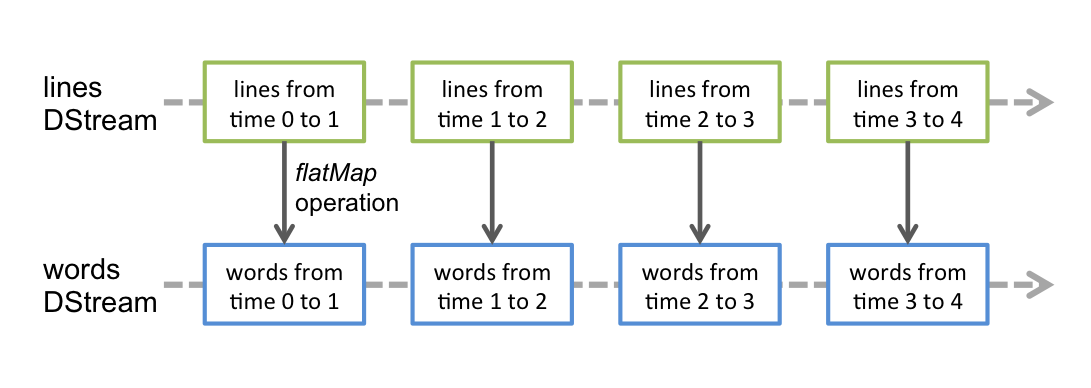
\includegraphics[scale=0.7]{streaming-dstream-ops}  
	\caption[Gambar mengubah{\it Data Stream} dari lines ke words]{mengubah{\it Data Stream} dari lines ke words} 
	\label{fig:processing-events relationship} 
	\end{figure}
	
\textit{DStream} dapat dibuat dari sumber eksternal ataupun menggunakan hasil transformasi dari \textit{Dstream} lain. \textit{DStream} juga memiliki  \textit{Stateful transformations} yang bisa mengagregasi data pada seluruh interval yang ada. pembahasan tentang \textit{stateful transformation} akan dibahas lebih jelas di bab berikutnya.

Untuk setiap sumber input, \textit{spark streaming} meluncurkan \textit{recievers} yang mana adalah \textit{task} yang berjalan pada eksekutor yang mengumpulkan data dari sumber input dan menyimpannya sebagai RDD. Selain menyimpan data, \textit{recievers} juga mereplikasi data ke eksekutor lain untuk mencapai \textit{fault-tolerance}. Data akan disimpan di memori eksekutor sama seperi \textit{cache} pada RDD. \textit{Receivers} juga bisa mereplikasi data ke HDFS. \textit{Streaming Context} pada \textit{driver} than secara periodik menjalankan \textit{Spark Jobs} untuk memproses data dan menggabungkannya dengan RDD sebelumnya.
  
\begin{figure}[H] 
	\centering  
	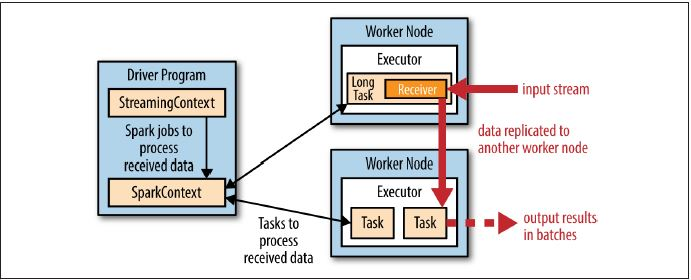
\includegraphics[scale=1]{spark-streaming-execution}  
	\caption[Gambar eksekusi{\it Spark Streaming} pada komponen \textit{Spark}]{eksekusi{\it Spark Streaming} pada komponen \textit{Spark}} 
	\label{fig:processing-events relationship} 
	\end{figure}

\textit{Spark Streaming} memiliki sifat \textit{fault-tolerant} yang sama dengan \textit{Spark} untuk RDD selama replika input data masih tersedia. \textit{Spark Streaming} bisa mengkomputasi ulang setiap \textit{state} yang diturunkan dari \textit{lineage}suatu RDD dengan cara menjalankan kembali operasi yang memproses RDD tersebut. Biasanya, data yang diterima direplika dalam dua node sehingga \textit{spark streaming} bisa mentoleransi satu worker yang gagal. Namun, jika menggunakan \textit{lineage} penghitungan ulang bisa memerlukan waktu yang lama karena datanya telah dibuat duluan. Karena itu, \textit{Spark Streaming} menyediakan mekanisme yang disebut \textit{checkpointing} yang akan menyimpan state secara berkala ke suatu file system seperti HDFS. \textit{checkpointing} akan dijalankan setiap lima atau sepuluh \textit{batch}. Ketika terjadi ingin memperbaiki data yang gagal \textit{Spark Streaming} hanya perlu kembali ke \textit{checkpoint} paling baru. 


 
\subsubsection{Transformasi}
Transformasi pada \textit{Spark Streaming} dikelompokan menjadi dua yaitu; \textit{stateless} atau \textit{Stateful}:
\begin{itemize}
	\item{ Pada transformasi \textit{stateless}, pemrosesan setiap batch tidak bergantung pada 		data di batch sebelumnya. Transformasi ini memiliki transformasi RDD seperti 					\texttt{map()},\texttt{reduce()}, dan \texttt{reduceByKey()}	
	}
	
	\item{Transformasi \textit{stateful} menggunakan data yang dihasilkan oleh \textit{batch} 		sebelumnya 	untuk menghitung hasil dari \textit{batch} saat ini. Transformasi ini memiliki 		\textit{sliding windows} dan bisa mengecek waktu pada seluruh interval.
	
	}
\end{itemize}

\begin{itemize}
	\item[]{\textbf{Stateless Transformations}\newline
	Transformasi \textit{Stateless} adalah transformasi RDD sederhana yang diterapkan kepada 		setiap RDD pada \textit{Dstreams}. Walaupun setiap fungsi terlihat diterapkan ke pada seluruh aliran data. Namun, secara internal setiap \textit{DStream} tersusun dari beberapa RDD (\textit{batches}) dan setiap transformasi \textit{stateless} diterapkan secara terpisah untuk setiap RDD. Contohnya, 
	 \texttt{reduceByKey()} akan melakukan \textit{reduce} pada data pada setiap \textit{batch 		 interval}. Untuk menggabungkan data pada seluruh interval diperlukan \textit{Stateful 			 Transformation} .
	 }
	
	\item[]{\textbf{\textit{Stateful Transformation}}\newline
	\textit{Stateful Transformation} adalah sebuah operasi pada \textit{Dstream} yang bisa 			menelusuri waktu pada semua interval sehingga data pada \textit{batch} sebelumnya bisa 			digunakan untuk \textit{batch} saat ini.\newline
	\textit{Spark Streaming} memerlukan \textit{checkpointing} untuk bisa diaktifkan di 			\textit{streaming context} sebagai upaya menghindari kesalahan \textit{fault}. 
	}
	
	\item[]{\textbf{\textit{Windowed Transformation}}\newline
		Transformasi ini menghitung hasil pada interval yang lebih lama dari \textit{streaming 					context} dengan menggabungkan beberapa \textit{batch} pada interval tertentu.
		pada transformasi \textit{windowing} ada tiga interval yang digunakan: \textit{batch, 					slide}, dan \textit{window interval}. 
		\textit{Batch Interval} adalah seberapa sering suatu data diambil ke dalam \textit{Dstream}. 		Durasi dari batch interval sangat sebentar setengah sampai satu detik. \textit{Batch time} 				tidak berkorelasi dengan apa yang akan dianalisis nanti. \textit{Batch Interval} hanya 					mengambil data sebanyak dan secepat mungkin dari suatu sumber data. \newline
		
		\begin{figure}[H] 
		\centering  
		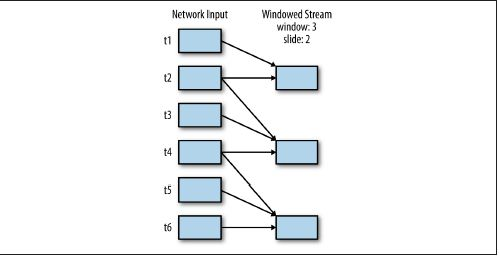
\includegraphics[scale=0.7]{windowing-streaming}  
		\caption[Gambar cara kerja \textit{Windowed Transformation}]{Gambar cara kerja 							\textit{Windowed Transformation}} 
		\label{fig:processing-events relationship} 
		\end{figure}
	}
		
\textit{Slide Interval} adalah titik acuan seberapa sering suatu informasi ingin 				dikomputasi, dan \textit{Window Interval} adalah bagaimana \textit{Spark Streaming} 			melihat ke belekang setiap kali bertemu dengan \textit{slide Interval}.

\end{itemize}


\subsubsection{Output Operations}
\textit{Output Operation} adalah fungsi akhir dari rantaian transformasi. Fungsi ini menentukan apa yang perlu dilakukan dengan data yang ditransformasikan pada akhir aliran. contoh: tampilkan ke layar atau simpan di database eksternal.

fungsi \textit{Output Operation} yang paling umum adalah \texttt{print()}. Fungsi ini menampilkan
10 element pada tiap \textit{batch} sebagai hasil. selain itu ada \texttt{saveAsTextFile("dir",name)} fungsi ini akan menyimpan hasil transformasi ke direktori yang telah ditentukan. Terakhir, ada \texttt{foreachRDD()}. Fungsi ini hampir sama dengan transform dimana kita memiliki akses pada setiap RDD. Sebagai contoh jika ingin menyimpan ke ekternal tabel \textit{MySQL} tidak bisa menggunakan \textit{SaveAs} tetapi harus mengakses tiap RDD dan memasukannya ke tabel \textit{MySQL} secara manual.
 
\subsubsection{Checkpointing}
\textit{Checkpointing} adalah mekanisme utama sebagai penyedia \textit{fault tolerance} untuk \textit{Spark Streaming}. Mekanisme ini memungkinkan \textit{sparkstreaming} untuk menyimpan data
secara periodik pada suatu \textit{storage system} seperti HDFS. Data yang disimpan ini adalah \textit{backup dari data asli}. Tujuan meyimpan data backup adalah:

\begin{itemize}
	\item mengurangi transformasi atau state yang harus dikomputasi ulang jika terjadi kegagalan.
	\textit{Spark Streaming} bisa mengkomputasi ulang data yang hilang dengan lineage graph.Tetapi,
	\textit{checkpointing} yang menentukan seberapa jauh lineage graph harus mengambil data. 
\end{itemize}

\begin{lstlisting}[language=Scala, caption= contoh checkpointing]
	ssc.checkpoint("hdfs://...")
\end{lstlisting}


\section{Input Sources}
\textit{Input Source} adalah penyedia data yang bisa terhubung dengan \textit{Spark Streaming}. \textit{Input Source} adalah komponen terpisah dari \textit{Spark Streaming} walaupun masih bagian dari \textit{Spark}. Untuk mengintegrasikan dengan \textit{Spark Streaming} dibutuhkan beberapa tambahan \textit{package} yang harus diikutsertakan pada \textit{build} file. Beberapa Input Source
adalah Twitter dan Kafka:

\subsection{Twitter API}
Twitter API adalah sekumpulan URL yang digunakan untuk mengakses data pada twitter tanpa melewati
antar muka web. URL akan digunakan sebagai parameter kode program nanti. data yang diambil pada twitter berupa objek. seperti contoh gambar:

\begin{figure}[H] 
	\centering  
	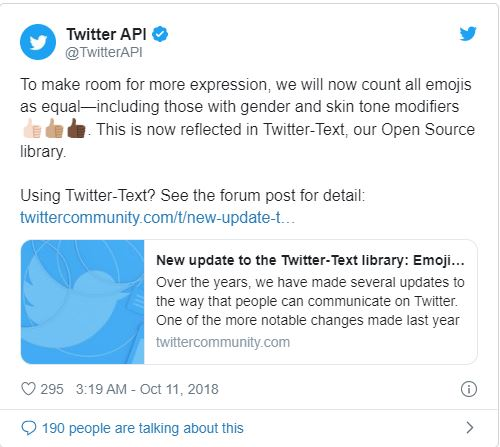
\includegraphics[scale=0.8]{twitter-object}  
	\caption[Gambar Twitter Object]{\textit{Twitter Object}} 
	\label{fig:Hadoop-home} 
\end{figure}

objek yang diakses akan disimpan dengan format JSON. Objek terdiri dari informasi-informasi yang membangun tweet seperti; tanggal berapa suatu tweet dibuat, id twitter yang menunggah tweet tersebut, isi pesan yang diunggah oleh pengguna(status), informasi pengguna itu sendiri, dan entitas luar yang ikut di dalam suatu tweet seperti link url atau mention. Berikut adalah contoh format JSON yang membangun suatu Tweet:

\begin{figure}[H] 
	\centering  
	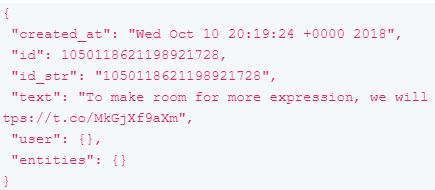
\includegraphics[scale=1]{twitterJSON}  
	\caption[Gambar Twitter Object]{\textit{Twitter Object JSON}} 
	\label{fig:Hadoop-home} 
\end{figure}

Informasi tentang pengguna terdiri dari beberapa objek lagi.Objek yang dimuat berupa id user, nama,
lokasi, url, deskripsi, status verifikasi, jumlah follower, jumlah following, dan lokasi.
 
\begin{figure}[H] 
	\centering  
	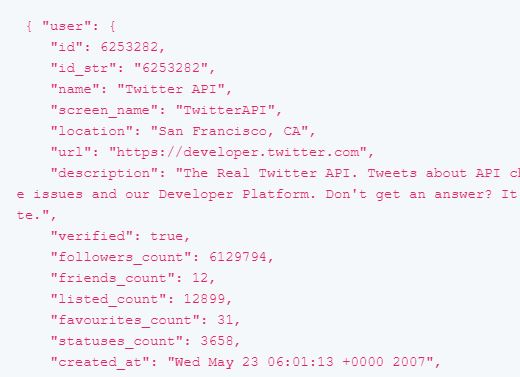
\includegraphics[scale=1]{userObject}  
	\caption[Gambar Twitter Object]{\textit{User Object JSON}} 
	\label{fig:Hadoop-home} 
\end{figure}

Namun dari beberapa banyak informasi yang terdapat pada twitter seseorang tidak semuanya bisa diakses hal ini bergantung ke pada kebijakan dari twitter dan persetujuan dari user. salah satu contohnya adalah lokasi seseorang. Lokasi seseorang hanya bisa diakses ketika user bersedia untuk menampilkan lokasi tersebut.

\subsection{Kafka}
 
\subsubsection{Konsep Publish/Messaging}
Sebelum membahas Kafka, penting untuk mengerti tentang sistem pengiriman \textit{publish/messaging} dan mengapa konsep ini sangat penting. \textit{publish/subscribe messaging} adalah \textit{pattern} yang dicirikan oleh pengirim \textit{publisiher} tidak langsung mengirimkannya ke penerima. Tetapi, pengirim mempublikasikan data yang dimiliki ke sebuah sistem lain yang disebut \textit{broker}, sebuah titik sentral di mana suatu pesan selalu diunggah. Sehingga penerima pesan bisa langsung mengikuti perkembangan data dan informasi yang dimiliki \textit{publisher} di broker. Penerima disebu \textit{Subscriber}.

\begin{figure}[H] 
	\centering  
	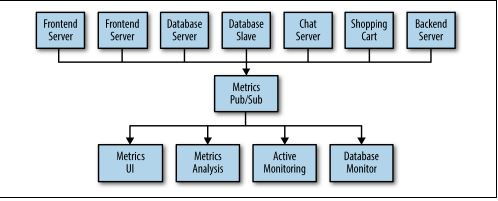
\includegraphics[scale=1]{pubsub}  
	\caption[Gambar Publisher/Subscriber]{\textit{Publisher/Subscriber}} 
	\label{fig:pub-sub} 
\end{figure}

seperti gambar di atas semua server mengirimkan data ke broker \textit{metrics} dan sistem-sistem yang ingin memilki data yang ingin diakses harus diintegrasikan dengan broker. Sistem-sistem tersebut mengikuti perkembangan dan perubahan data yang terjadi melalui broke (subscribe).

\subsubsection{Pengertian Kafka}
kafka adalah sebuah sistem pengriman data \textit{Publish/subscribe} yang didesain untuk menyelesaikan masalah yang sering disebut dengan \textit{distributed commit log} yang mana suatu \textit{filesystem} atau database didesain untuk menyediakan data rekord-rekord yang disimpan dengan lama dan bisa diakses kembali secara berkala pada sistem yang stabil. Data pada kafka disimpan dengan lama dan terurut. Berikut dalah komponen-komponen dari kafka:
 
\subsubsection{Messages and Batches} 
 Satuan data di kafka disebut dengan \textit{message}. \textit{Message} hampir sama seperti \textit{row} atau \textit{rekord}. Sebuah \textit{message} adalah array dari sekumpulan bytes karena itu \textit{message} pada kafka tidak memiliki format spesifik atau arti bagi kafka. Suatu \textit{message} bisa memiliki metadata yang disebut dengan \textit{key}. Untuk lebih efisien semua \textit{messages} ditulis pada \textit{batch}. \textit{batch} adalah sekumpulan pesan yang diproduksi oleh topik dan partisi yang sama. 
 
\subsubsection{Schemas}
Kakfa mengetahui \textit{message} adalah sebuah \textit{array of bytes}. Sehingga kafka membutuhkan skema atau struktur yang diterapkan pada pesan sehinggga bisa mudah dimengerti. Ada banyak cara untuk menerapkan skema tergantung kebutuhan aplikasi. Contoh dari skema bisa berbentuk JSON atau XML
sehingga manusia bisa membaca pesan yang ada pada kafka.


\subsubsection{Topics}
\textit{Message} pada kafka disebut sebagai \textit{topics}. \textit{Topics} adalah sebuah kategori atau sebuah nama \textit{feed} dimana suatu rekord dipublikasi. Analoginya, topik adalah tabel basis data atau suatu folder di filesystem. Suatu rekord bisa disimpan di folder atau basis data dengan identifikasi pengenal.

\begin{figure}[H] 
	\centering  
	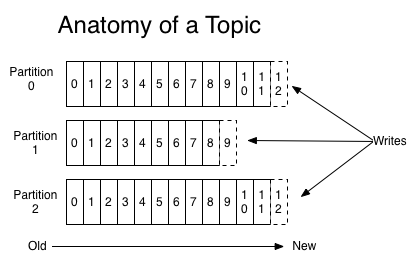
\includegraphics[scale=1]{kafkatopic}  
	\caption[Gambar Topic pada Kafka]{\textit{Topic pada kafka}} 
	\label{fig:kafka-topic} 
\end{figure}
Setiap partisi adalah sebuah sekuensi yang terurut, tidak bisa diubah-ubah \textit{immutable} yang terus ada pada \textit{commit log}. Setiap rekord pada p\textit{partition} diberi tanda dengan nomer sekuensial yang disebut offset yang menandai rekord secara unik. Partition adalah tempat dimana topic disimpan.

Klaster pada kafka akan terus menyimpan topic terlepas topik itu digunakan atau tidak selama waktu yang telah ditentukan \textit{(retention period)}. Contoh jika suatu \textit{retention period} pada topic diatur menjadi 2 hari maka topic tersebut akan ada selama dua hari dan tidak bisa dihapus pada interval waktu itu. Sehingga setiap \textit{subscriber} masih bisa mengakses data tersebut. Setelah itu baru dihapus.

\begin{figure}[H] 
	\centering  
	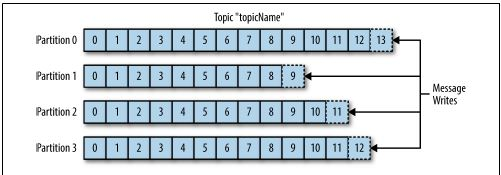
\includegraphics[scale=1]{streamtopic}  
	\caption[Gambar stream topic]{\textit{stream topic}} 
	\label{fig:kafka-stream} 
\end{figure}

Begitu juga dengan \textit{data stream}. Pada kafka, \textit{Data Stream} dianggap sebagai satu topic terlepas dari banyak partisi. Sebagai contoh keempat partisi pada gambar di atas masih disebut sebagai satu stream.

\subsubsection{Producers and Consumers}
Pengguna yang menggunakan sistem kafka disebut dengan klien. Ada dua tipe kline \textit{producer} dan \textit{consumer}. Bisa juga kakfa diintegrasikan dengan sistem API lain. Tugas dari \textit{producer} adalah membuat \textit{membuat message} dan mengirimnya ke \textit{topic} tertentu pada broker. \textit{Consumer} adalah yang membaca pesan degan cara mengakses topic-topic tertentu pada broker.

\subsubsection{Broker}  
 Sebuah kafka server disebut dengan broker. Sebuah broker menerima pesan dari \textit{producer} memberi \textit{offset} pada pesan tersebut dan menyimpannya pada sebuah disk. Broker juga berinteraksi dengan \textit{consumer} ketika konsumer meminta akses pada suatu partisi dan membalas \textit{consumer} dengan pesan yang diinginkan dan ada di disk.
 
 \begin{figure}[H] 
	\centering  
	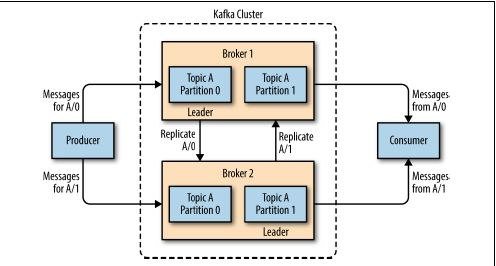
\includegraphics[scale=1]{replikasibroker}  
	\caption[Gambar Kafka Broker]{Kafka Broker} 
	\label{fig:kafka-broker} 
\end{figure}

 \textit{Broker} dirancang untuk berjalan pada klaster. Dari rangkaian \textit{broker} pada klaster
 satu \textit{broker} akan bertindak sebagai \textit{controller} yang dipilih secara otomatis dan berfungsi untuk mengatur operasi administratif seperti; menentukan partisi mana topic akan disimpan atau mengawasi jika terjadi \textit{failure} pada broker lain. Sebuah partisi bisa disimpan pada dua broker secara bersamaan.
 
    
\label{sec:ApacheSpark}


%Berikut adalah contoh pembuatan tabel. 
%Penempatan tabel dan gambar secara umum diatur secara otomatis oleh \LaTeX{}, perhatikan contoh di file bab2.tex untuk melihat bagaimana cara memaksa tabel ditempatkan sesuai keinginan kita.
%
%Perhatikan bawa berbeda dengan penempatan judul gambar gambar, keterangan tabel harus diletakkan di atas tabel!!
%Lihat Tabel~\ref{tab:contoh1} berikut ini:
%
%\begin{table}[H] %atau h saja untuk "kira kira di sini"
%	\centering 
%	\caption{Tabel contoh}
%	\label{tab:contoh1}
%	\begin{tabular}{cccc}
%		\toprule
%		& $v_{start}$ & $\mathcal{S}_{1}$ & $v_{end}$\\
%
%		\midrule
%		$\tau_{1}$ & 1 & 12& 20\\
%		$\tau_{2}$ & 1 &  & 20\\
%		$\tau_{3}$ & 1 & 9 & 20\\
%		$\tau_{4}$ & 1 &  & 20\\
%
%		\bottomrule
%		
%	\end{tabular} 
%\end{table}
%Tabel~\ref{tab:cthwarna1} dan Tabel~\ref{tab:cthwarna2} berikut ini adalah tabel dengan sel yang berwarna dan ada dua tabel yang bersebelahan. 
%\begin{table}[H]
%	\begin{minipage}[c]{0.49\linewidth}
%		\centering
%		\caption{Tabel bewarna(1)}
%		\label{tab:cthwarna1}
%		\begin{tabular}{ccccc}
%			\toprule
%			 & $v_{start}$ & $\mathcal{S}_{2}$ & $\mathcal{S}_{1}$ & $v_{end}$\\
%			
%			\midrule
%			$\tau_{1}$ & 1 & 5 \cellcolor{green}& 12& 20\\
%			$\tau_{2}$ & 1 & 8 \cellcolor{green}& & 20\\
%			$\tau_{3}$ & 1 & 2/8/17 \cellcolor{green}& 9 & 20\\
%			$\tau_{4}$ & 1 & \cellcolor{red}& & 20\\
%			
%			\bottomrule
%
%		\end{tabular}
%	\end{minipage}
%	\begin{minipage}[c]{0.49\linewidth}
%		
%		\centering 
%		\caption{Tabel bewarna(2)}
%		\label{tab:cthwarna2}
%		\begin{tabular}{ccccc}
%			\toprule
%			 & $v_{start}$ & $\mathcal{S}_{1}$ & $\mathcal{S}_{2}$ & $v_{end}$\\
%			
%			\midrule
%			$\tau_{1}$ & 1 & 12& 5 \cellcolor{red} &20\\
%			$\tau_{2}$ & 1 &  &  8 \cellcolor{green} &20\\
%			$\tau_{3}$ & 1 & 9 & 2/8/17 \cellcolor{green} &20\\
%			$\tau_{4}$ & 1 &   & \cellcolor{red} &20\\
%			
%			\bottomrule
%		
%		\end{tabular}
%	\end{minipage}
%\end{table}

 
%\section{Kutipan}
%Berikut contoh kutipan dari berbagai sumber, untuk keterangan lebih lengkap, silahkan membaca file %referensi.bib yang disediakan juga di template ini.
%Contoh kutipan:
%\begin{itemize}
%	\item Buku:~\cite{berg:08:compgeom} 
%	\item Bab dalam buku:~\cite{kreveld:04:GIS}
%	\item Artikel dari Jurnal:~\cite{buchin:13:median}
%	\item Artikel dari prosiding seminar/konferensi:~\cite{kreveld:11:median}
%	\item Skripsi/Thesis/Disertasi:~\cite{lionov:02:animasi}~\cite{wiratma:10:following}~%\cite{wiratma:22:later}
%	\item Technical/Scientific Report:~\cite{kreveld:07:watertight}
%	\item RFC (Request For Comments):~\cite{RFC1654}
%	\item Technical Documentation/Technical Manual:~\cite{Z.500}~\cite{unicode:16:stdv9}~%\cite{google:16:and7}
%	\item Paten:~\cite{webb:12:comm}
%	\item Tidak dipublikasikan:~\cite{wiratma:09:median}~\cite{lionov:11:cpoly}
%	\item Laman web:~\cite{erickson:03:cgmodel}  
%	\item Lain-lain:~\cite{agung:12:tango}
%\end{itemize}    
%\label{subs:kutipan} 
%\subsection{Gambar}

%Pada hampir semua editor, penempatan gambar di dalam dokumen \LaTeX{} tidak dapat dilakukan melalui proses {\it drag and drop}.
%Perhatikan contoh pada file bab2.tex untuk melihat bagaimana cara menempatkan gambar.
%Beberapa hal yang harus diperhatikan pada saat menempatkan gambar:
%\begin{itemize}
%	\item Setiap gambar {\bf harus} diacu di dalam teks (gunakan {\it field} {\sc label})
%	\item {\it Field} {\sc caption} digunakan untuk teks pengantar pada gambar. Terdapat dua bagian yaitu yang ada di antara tanda $[$ dan $]$ dan yang ada di antara tanda $\{$ dan $\}$. Yang pertama akan muncul di Daftar Gambar, sedangkan yang kedua akan muncul di teks pengantar gambar. Untuk skripsi ini, samakan isi keduanya.
%	\item Jenis file yang dapat digunakan sebagai gambar cukup banyak, tetapi yang paling populer adalah tipe {\sc png} (lihat Gambar~\ref{fig:ularpng}), tipe {\sc jpg} (Gambar~\ref{fig:ularjpg}) dan tipe {\sc pdf} (Gambar~\ref{fig:ularpdf})
%	\item Besarnya gambar dapat diatur dengan {\it field} {\sc scale}.
%	\item Penempatan gambar diatur menggunakan {\it placement specifier} (di antara tanda  $[$ dan $]$ setelah deklarasi gambar.
%	Yang umum digunakan adalah {\bf H} untuk menempatkan gambar {\bf sesuai} penempatannya di file .tex atau  {\bf h} yang berarti "kira-kira" di sini. \\
%	Jika tidak menggunakan {\it placement specifier}, \LaTeX{} akan menempatkan gambar secara otomatis untuk menghindari bagian kosong pada dokumen anda.
%	Walaupun cara ini sangat mudah, hindarkan terjadinya penempatan dua gambar secara berurutan. 	
%	\begin{itemize}
%		\item Gambar~\ref{fig:ularpng} ditempatkan di bagian atas halaman, walaupun penempatannya dilakukan setelah penulisan 3 paragraf setelah penjelasan ini.
%		\item Gambar~\ref{fig:ularjpg} dengan skala 0.5 ditempatkan di antara dua buah paragraf. Perhatikan penulisannya di dalam file bab2.tex!
%		\item Gambar~\ref{fig:ularpdf} ditempatkan menggunakan {\it specifier} {\bf h}.
%	\end{itemize}
%\end{itemize}
% 
%\dtext{17-18}
%\begin{figure} 
%	\centering  
%	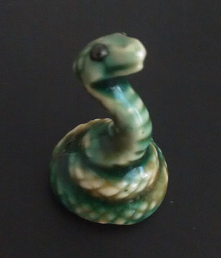
\includegraphics[scale=1]{ular-png}  
%	\caption[Gambar {\it Serpentes} dalam format png]{Gambar {\it Serpentes} dalam format png} 
%	\label{fig:ularpng} 
%\end{figure} 
%
%\dtext{19-20}
%\begin{figure}[H]
%	\centering  
%	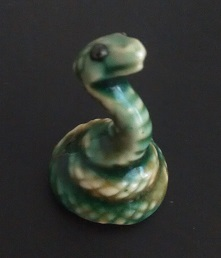
\includegraphics[scale=0.5]{ular-jpg}  
%	\caption[Ular kecil]{Ular kecil} 
%	\label{fig:ularjpg} 
%\end{figure} 
%\dtext{21-22}
%
%\begin{figure}[ht] 
%	\centering  
%	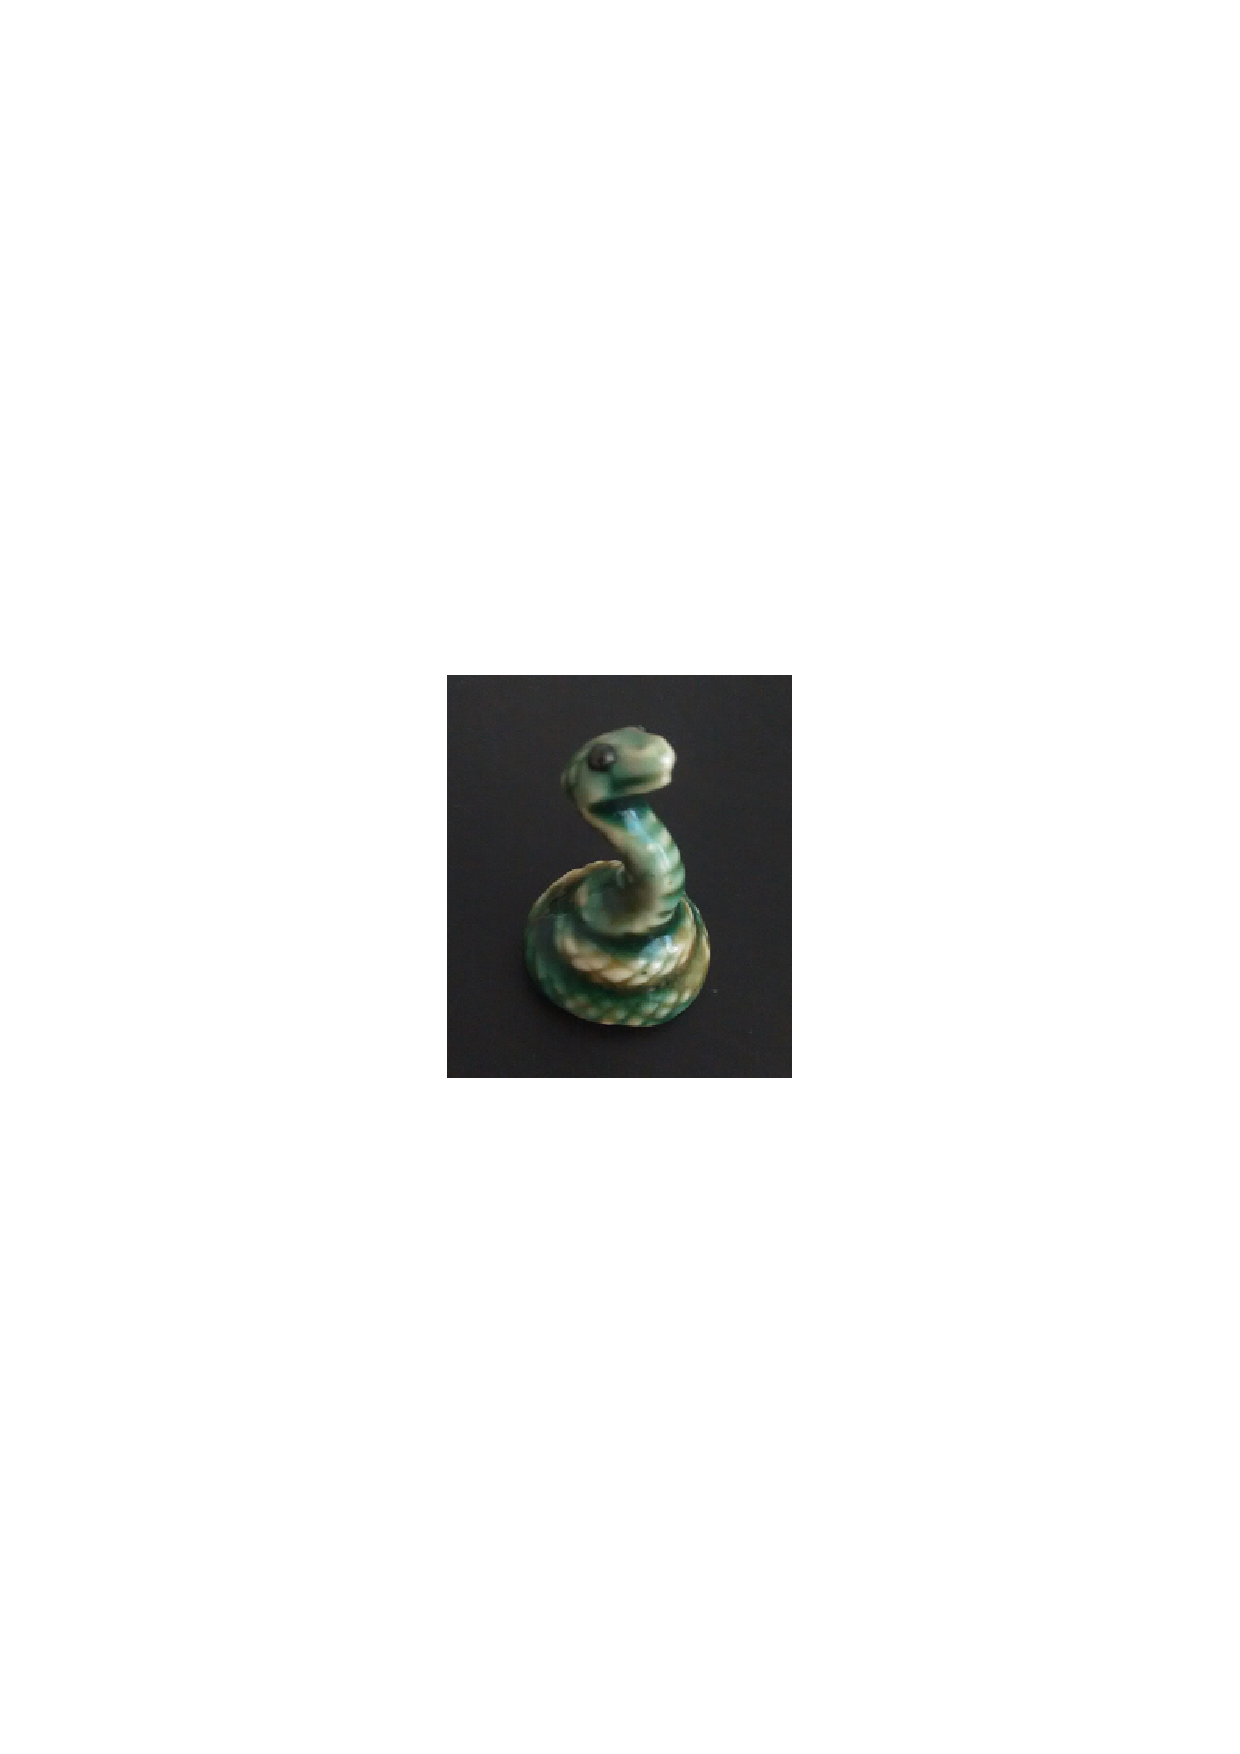
\includegraphics[scale=1]{ular-pdf}  
%	\caption[ {\it Serpentes} betina]{ {\it Serpentes} jantan} 
%	\label{fig:ularpdf} 
%\end{figure} 
%
%\label{sec:Twitter} 
